\documentclass[12pt]{book}
\usepackage[utf8]{inputenc}
\usepackage{amsmath}
\usepackage{amsfonts}
\usepackage{amssymb}

\usepackage{graphicx}
\usepackage{xcolor}
\usepackage{tikz}
\usetikzlibrary{shapes.geometric, arrows, positioning}
\usepackage{tabularx}
\usepackage{array}
\usepackage{lipsum}
\usepackage{hyperref}
\usepackage{pgfplots}
\usepackage{ifthen} % Make sure to include this for ifthenelse
\usepackage{tikz}
\usepackage{caption}
\pgfplotsset{compat=1.18}
\hypersetup{
    colorlinks=true,
    linkcolor=blue,
    filecolor=magenta,      
    urlcolor=cyan,
    pdftitle={Overleaf Example},
    pdfpagemode=FullScreen,
    }

\urlstyle{same}
\definecolor{myblue}{RGB}{77,148,255}
\definecolor{mygreen}{RGB}{167,225,89}
\definecolor{myred}{RGB}{255,110,110}

\newcommand{\mybox}[2]{%
  \noindent
  \begin{center}
    \begin{tikzpicture}
      \node[rectangle, rounded corners, fill=#1!20, draw=#1, text width=0.9\textwidth, inner sep=10pt, align=left] (box)  {#2};
    \end{tikzpicture}
  \end{center}
}


\begin{document}
\title{Ace Your HAM Radio Extra Class Exam}
\author{Charles Perng}
\date{\today}
\maketitle

\frontmatter
\tableofcontents

\mainmatter

%% ************************************************************************
% CHAPTER 1: Sublement E1 - Commission Rules
% ************************************************************************
\chapter{E1: Commission Rules}

% ------------------------------------------------------------------------
% SECTION E1A: Frequency Privileges and Band Restrictions
% ------------------------------------------------------------------------
\section{E1A: Frequency Privileges and Band Restrictions}

\subsection*{Understanding the Basics}
  \textcolor{myblue}{\textbf{Frequency privileges}} in amateur radio refers to the specific ranges of radio frequencies that licensed amateur operators are allowed to use. These bands are not random; they are allocated by international and national regulatory bodies. Each band has different propagation characteristics that make them suitable for different types of communication.
  \par
  \textcolor{myblue}{\textbf{Power restrictions}} dictate how much output power your transmitter can use. These are also band-specific. Some bands, like 630- and 2200-meter bands, have lower power limits due to their unique propagation and interference potential.
  \par
  It is very important that all users operate within allocated bands and power restrictions for that band.
  
\mybox{mygreen}{
  \textbf{Fun Fact}: The 630-meter and 2200-meter bands are relatively new additions to the US amateur radio allocation, offering hams a taste of "low-band" propagation!  These bands have unique challenges and opportunities for experimentation, allowing for long-distance communications through ground-wave and sky-wave propagation. They also require notifications and special operating procedures.
  }
  
\subsection*{Key Concepts for the Questions}
\begin{itemize}
    \item \textbf{HF (High Frequency) Bands:} These range from approximately 3 to 30 MHz and offer various long-distance communications opportunities.
    \item \textbf{Band Edges:}  The upper and lower limits of a specific frequency band.
    \item \textbf{USB/LSB (Upper Sideband/Lower Sideband):} Two common modes of transmission in the HF bands. They are different types of Amplitude Modulation where carrier is suppressed and only one side band is transmitted. In general Upper Sideband is used for bands with a central frequency of above 10 MHz and LSB is used otherwise.
    \item \textbf{Phone Mode:} The modulation for carrying voice. It often uses single side band.
    \item \textbf{Data Mode}: A wide variety of modulation used for digital data transmissions.
    \item \textbf{Carrier Frequency:} The base frequency at which a radio signal is transmitted.
    \item \textbf{Bandwidth:} The range of frequencies that a signal occupies.
\end{itemize}

\subsection*{Practice Questions}
\begin{enumerate}
    \item Why is it not legal to transmit a 3 kHz bandwidth USB signal with a carrier frequency of 14.348 MHz?
    \begin{enumerate}
        \item USB is not used on 20-meter phone
        \item  The lower 1 kHz of the signal is outside the 20-meter band
        \item  14.348 MHz is outside the 20-meter band
        \item  \textbf {The upper 1 kHz of the signal is outside the 20-meter band}
    \end{enumerate}
    \textcolor{myred}{Explanation:}
    The 20-meter amateur band is roughly from 14.000 to 14.350 MHz. When transmitting in USB mode, the carrier frequency is at the bottom of transmitted signal. For 3 KHz signal, the top of the signal is at 14.351 MHz which is out of the permitted band, therefore is not legal.
        
    \item When using a transceiver that displays the carrier frequency of phone signals, which of the following displayed frequencies represents the lowest frequency at which a properly adjusted LSB emission will be totally within the band?
    \begin{enumerate}
        \item The exact lower band edge
        \item  300 Hz above the lower band edge
        \item  1 kHz above the lower band edge
        \item \textbf {3 kHz above the lower band edge}
    \end{enumerate}
    \textcolor{myred}{Explanation:}
    When transmitting in LSB mode, the carrier frequency is at the top of the transmitted signal. For a 3 kHz bandwidth signal, the lower end will be 3 kHz below the displayed frequency. For the signal to be in the band, the lowest end of the signal needs to be at the band edge. Thus the displayed carrier frequency should be 3 kHz above the band edge.
    
        \item What is the highest legal carrier frequency on the 20-meter band for transmitting a 2.8 kHz wide USB data signal?
    \begin{enumerate}
        \item 14.0708 MHz
         \item  14.1002 MHz
         \item \textbf {14.1472 MHz}
        \item  14.3490 MHz
    \end{enumerate}
    \textcolor{myred}{Explanation:}
    The highest end of 20m band is 14.350 MHz. Because we are using USB mode, our carrier frequency will be on the lower end of the signal, thus, the carrier can go up to 14.350 MHz - 2.8 KHz = 14.3472 MHz. The data portion of the 20 meter band ends at 14.150 MHz. The highest legal carrier frequency is then 14.150 MHz-0.0028 MHz = 14.1472 MHz.

    
        \item May an Extra class operator answer the CQ of a station on 3.601 MHz LSB phone?
    \begin{enumerate}
        \item Yes, the entire signal will be inside the SSB allocation for Extra class operators
        \item  Yes, the displayed frequency is within the 75-meter phone band segment
        \item \textbf {No, the sideband components will extend beyond the edge of the phone band segment}
         \item  No, US stations are not permitted to use phone emissions below 3.610 MHz
        \end{enumerate}
         \textcolor{myred}{Explanation:}
          Extra class operators have voice allocation above 3.600 MHz. The lowest edge of the phone segment is 3.600 MHz. If we are using LSB and transmitting at 3.601 MHz, the lower side band goes below 3.600 MHz. Thus, the signal will extend beyond the band edge and become illegal.
          
      \item Who must be in physical control of the station apparatus of an amateur station aboard any vessel or craft that is documented or registered in the United States?
\begin{enumerate}
   \item Only a person with an FCC Marine Radio license grant
\item  Only a person named in an amateur station license grant
\item \textbf {Any person holding an FCC issued amateur license or who is authorized for alien reciprocal operation}
\item  Any person named in an amateur station license grant or a person holding an unrestricted Radiotelephone Operator Permit
\end{enumerate}
\textcolor{myred}{Explanation:}
Any licensed amateur operator can operate the station on a vessel or aircraft. There is no need for any special endorsement.
 
    \item What is the required transmit frequency of a CW signal for channelized 60 meter operation?
    \begin{enumerate}
        \item At the lowest frequency of the channel
        \item \textbf {At the center frequency of the channel}
        \item  At the highest frequency of the channel
        \item  On any frequency where the signal's sidebands are within the channel
    \end{enumerate}
     \textcolor{myred}{Explanation:}
    The 60-meter band has specific channels and each channel has center frequencies for CW operations.

    \item What is the maximum power permitted on the 2200-meter band?
    \begin{enumerate}
        \item 50 watts PEP (peak envelope power)
        \item  100 watts PEP (peak envelope power)
         \item \textbf {1 watt EIRP (equivalent isotropic radiated power)}
        \item  5 watts EIRP (equivalent isotropic radiated power)
    \end{enumerate}
    \textcolor{myred}{Explanation:}
     The 2200 meter band is among the newest allocations and has special restrictions, including the use of EIRP for power limitation, that is different from the traditional PEP method.

      \item If a station in a message forwarding system inadvertently forwards a message that is in violation of FCC rules, who is primarily accountable for the rules violation?
    \begin{enumerate}
        \item The control operator of the packet bulletin board station
        \item \textbf {The control operator of the originating station}
        \item  The control operators of all the stations in the system
        \item  The control operators of all the stations in the system not authenticating the source from which they accept communications
    \end{enumerate}
      \textcolor{myred}{Explanation:}
     The control operator of the originating station is responsible for ensuring the contents of any transmission is within FCC regulations, regardless of how it is forwarded.
       
      \item Except in some parts of Alaska, what is the maximum power permitted on the 630-meter band?
        \begin{enumerate}
       \item 50 watts PEP (peak envelope power)
      \item  100 watts PEP (peak envelope power)
       \item  1 watt EIRP (equivalent isotropic radiated power)
        \item \textbf {5 watts EIRP (equivalent isotropic radiated power)}
    \end{enumerate}
        \textcolor{myred}{Explanation:}
         The 630 meter band has special restrictions, including the use of EIRP for power limitation, that is different from the traditional PEP method.
         
      \item If an amateur station is installed aboard a ship or aircraft, what condition must be met before the station is operated?
        \begin{enumerate}
        \item \textbf {Its operation must be approved by the master of the ship or the pilot in command of the aircraft}
       \item  The amateur station operator must agree not to transmit when the main radio of the ship or aircraft is in use
       \item  The amateur station must have a power supply that is completely independent of the main ship or aircraft power supply
        \item  The amateur station must operate only in specific segments of the amateur service HF and VHF bands
     \end{enumerate}
        \textcolor{myred}{Explanation:}
    If operating on a ship or aircraft, the master or pilot must give approval before operating the station.
      
    \item What licensing is required when operating an amateur station aboard a US-registered vessel in international waters?
      \begin{enumerate}
     \item Any amateur license with an FCC Marine or Aircraft endorsement
    \item \textbf {Any FCC-issued amateur license}
       \item  Only General class or higher amateur licenses
     \item  An unrestricted Radiotelephone Operator Permit
      \end{enumerate}
     \textcolor{myred}{Explanation:}
      Any FCC issued amateur radio license will grant operator access on a US registered vessel in international water. There is no requirement for marine or aircraft endorsement.
\end{enumerate}


% ------------------------------------------------------------------------
% SECTION E1B: Station Restrictions and Special Operations
% ------------------------------------------------------------------------
\section{E1B: Station Restrictions and Special Operations}

\subsection*{Understanding the Basics}
  \textcolor{myblue}{\textbf{Station restrictions}} cover various aspects of your amateur radio operation. These can include limits on where you can set up a station, how high your antennas can be, what kind of emissions are permitted, and more. These restrictions are in place to minimize interference with other radio services and to ensure that your station operation doesn't negatively affect public safety.
  \par
  \textcolor{myblue}{\textbf{Spurious emissions}} are any emissions outside the intended bandwidth of your signal. This is important because these unwanted signals can interfere with other radio services. These are controlled by FCC regulations.
  \par
  \textcolor{myblue}{\textbf{RACES (Radio Amateur Civil Emergency Service)}} is a special operating program for amateur radio during emergencies. It often allows for use of restricted frequencies during emergencies. 
   \mybox{mygreen}{
      \textbf{Fun Fact}: Did you know that many of the rules and regulations that we follow today were developed based on a combination of historical precedence and new technological development? Regulations often balance the need for access to frequencies with the goal of minimizing interference, especially among essential services.
      }

\subsection*{Key Concepts for the Questions}
\begin{itemize}
    \item \textbf{Spurious Emissions:} Unwanted signals outside the necessary bandwidth of a transmission.
    \item \textbf{Necessary Bandwidth:} The minimum bandwidth required to transmit the information in a signal.
    \item \textbf{FCC Monitoring Facility:} A location where the Federal Communications Commission monitors radio activity.
    \item \textbf{RACES:} Radio Amateur Civil Emergency Service; a service providing emergency communications.
    \item \textbf{Public Use Airport:} An airport used by commercial and private aircraft.
    \item \textbf{PRB-1:}  A federal document that establishes guidelines for zoning regulations affecting amateur radio antennas.
    \item \textbf{Notam (Notice to Air Missions):}  A notice filed with FAA when construction of tall structures can become hazards to the air crafts
\end{itemize}

\subsection*{Practice Questions}
\begin{enumerate}
    \item Which of the following constitutes a spurious emission?
    \begin{enumerate}
        \item An amateur station transmission made without the proper call sign identification
        \item  A signal transmitted to prevent its detection by any station other than the intended recipient
        \item  Any transmitted signal that unintentionally interferes with another licensed radio station and whose levels exceed 40 dB below the fundamental power level
        \item \textbf {An emission outside the signal's necessary bandwidth that can be reduced or eliminated without affecting the information transmitted}
    \end{enumerate}
    \textcolor{myred}{Explanation:}
    A spurious emission is any emission from a transmitter that is outside its designed bandwidth, which can be eliminated without sacrificing the content of transmission.

     \item Which of the following is an acceptable bandwidth for digital voice or slow-scan TV transmissions made on the HF amateur bands?
    \begin{enumerate}
        \item \textbf {3 kHz}
        \item  10 kHz
        \item  15 kHz
        \item  20 kHz
    \end{enumerate}
       \textcolor{myred}{Explanation:}
   While there are some exception, 3 kHz is the most common limit for digital voice and slow-scan TV signals on the HF bands. This is to make sure those signal does not interfere with the other signals in the band.

       \item Within what distance must an amateur station protect an FCC monitoring facility from harmful interference?
       \begin{enumerate}
         \item \textbf {1 mile}
         \item  3 miles
         \item  10 miles
        \item  30 miles
        \end{enumerate}
        \textcolor{myred}{Explanation:}
    The FCC mandates that amateur stations must protect FCC monitoring facilities within 1 mile from harmful interference.
    
       \item What must the control operator of a repeater operating in the 70-centimeter band do if a radiolocation system experiences interference from that repeater?
       \begin{enumerate}
        \item Reduce the repeater antenna HAAT (Height Above Average Terrain)
         \item  File an FAA NOTAM (Notice to Air Missions) with the repeater system's ERP, call sign, and six-character grid locator
       \item \textbf {Cease operation or make changes to the repeater that mitigate the interference}
        \item  All these choices are correct
        \end{enumerate}
          \textcolor{myred}{Explanation:}
      The control operator must make changes to the repeater or cease the operation to mitigate interference with radiolocation.
        
         \item What is the National Radio Quiet Zone?
       \begin{enumerate}
          \item An area surrounding the FCC monitoring station in Laurel, Maryland
      \item  An area in New Mexico surrounding the White Sands Test Area
    \item \textbf {An area surrounding the National Radio Astronomy Observatory}
       \item  An area in Florida surrounding Cape Canaveral
        \end{enumerate}
          \textcolor{myred}{Explanation:}
       The National Radio Quiet Zone surrounds the National Radio Astronomy Observatory in West Virginia and limits certain radio transmissions.
       
        \item Which of the following additional rules apply if you are erecting an amateur station antenna structure at a site at or near a public use airport?
        \begin{enumerate}
        \item \textbf {You may have to notify the Federal Aviation Administration and register it with the FCC as required by Part 17 of the FCC rules}
       \item  You may have to enter the height above ground in meters, and the latitude and longitude in degrees, minutes, and seconds on the FAA website
         \item  You must file an Environmental Impact Statement with the EPA before construction begins
    \item  You must obtain a construction permit from the airport zoning authority per Part 119 of the FAA regulations
      \end{enumerate}
    \textcolor{myred}{Explanation:}
     Antenna construction near an airport must follow part 17 of the FCC rules and may require notification of FAA.
     
    \item To what type of regulations does PRB-1 apply?
      \begin{enumerate}
          \item Homeowners associations
       \item  FAA tower height limits
      \item \textbf {State and local zoning}
       \item  Use of wireless devices in vehicles
        \end{enumerate}
     \textcolor{myred}{Explanation:}
     PRB-1 is for zoning regulations and establish guidance for state and local zoning rules when regarding the construction of radio antennas.
    
       \item What limitations may the FCC place on an amateur station if its signal causes interference to domestic broadcast reception, assuming that the receivers involved are of good engineering design?
      \begin{enumerate}
          \item The amateur station must cease operation
      \item  The amateur station must cease operation on all frequencies below 30 MHz
         \item  The amateur station must cease operation on all frequencies above 30 MHz
      \item \textbf {The amateur station must avoid transmitting during certain hours on frequencies that cause the interference}
      \end{enumerate}
    \textcolor{myred}{Explanation:}
    If a station signal is causing interference with broadcasting reception, FCC can request avoidance of transmission in those frequencies when the interference is happening.
       
      \item Which amateur stations may be operated under RACES rules?
        \begin{enumerate}
          \item Only those club stations licensed to Amateur Extra class operators
       \item  Any FCC-licensed amateur station except a Technician class
     \item \textbf {Any FCC-licensed amateur station certified by the responsible civil defense organization for the area served}
     \item  Only stations meeting the FCC Part 97 technical standards for operation during an emergency
    \end{enumerate}
    \textcolor{myred}{Explanation:}
    Any FCC-licensed amateur radio can operate under RACES rules if certified by the local civil defense organization.
     
    \item What frequencies are authorized to an amateur station operating under RACES rules?
    \begin{enumerate}
      \item \textbf {All amateur service frequencies authorized to the control operator}
    \item  Specific segments in the amateur service MF, HF, VHF, and UHF bands
    \item  Specific local government channels
        \item  All these choices are correct
    \end{enumerate}
     \textcolor{myred}{Explanation:}
     A RACES operation may use all amateur radio bands and modes authorized to the control operator.
    
    \item What does PRB-1 require of state and local regulations affecting amateur radio antenna size and structures?
    \begin{enumerate}
        \item No limitations may be placed on antenna size or placement
        \item \textbf {Reasonable accommodations of amateur radio must be made}
        \item  Such structures must be permitted when use for emergency communications can be demonstrated
        \item  Such structures must be permitted if certified by a registered professional engineer
        \end{enumerate}
     \textcolor{myred}{Explanation:}
     PRB-1 dictates that zoning rules should be applied with reasonable accommodations for amateur radio.
\end{enumerate}

% ------------------------------------------------------------------------
% SECTION E1C: Automatic and Remote Control
% ------------------------------------------------------------------------
\section{E1C: Automatic and Remote Control}
\subsection*{Understanding the Basics}
  \textcolor{myblue}{\textbf{Automatic control}} refers to the operation of a ham radio station without the direct, active participation of a control operator. This can involve computer programs, timers, or other automation.
  \par
  \textcolor{myblue}{\textbf{Remote control}} involves operation of a station over a distance, typically using radio links or the internet. While remote operation provides great flexibility, it also requires careful attention to regulations.
  \par
  \textcolor{myblue}{\textbf{Band-specific regulations}} can be very different. It is essential to be familiar with these requirements.
   \par
  \textcolor{myblue}{\textbf{Spurious emission standards}} are very important to prevent interference to other communication services.
  \par
  \textcolor{myblue}{\textbf{HF modulation index limit}} is important for the voice operation, as explained in E8B.
  \par

  \subsection*{Deep Dive}
  
\subsubsection*{Modulation Index}

The \textbf{modulation index} is a measure of the extent of modulation in an amplitude modulation (AM) system. It is defined as the ratio of the amplitude of the modulating signal to the amplitude of the carrier signal. Mathematically, it is expressed as:

\begin{equation}
    m = \frac{A_m}{A_c}
\end{equation}

where:
\begin{itemize}
    \item $m$ is the modulation index,
    \item $A_m$ is the amplitude of the modulating signal,
    \item $A_c$ is the amplitude of the carrier signal.
\end{itemize}

The modulation index determines the characteristics of the AM signal:
\begin{itemize}
    \item \textbf{Under-Modulation:} $m < 1$, where the modulating signal is weaker than the carrier signal.
    \item \textbf{Critical Modulation:} $m = 1$, where the amplitude of the modulating signal equals the amplitude of the carrier signal.
    \item \textbf{Over-Modulation:} $m > 1$, where the modulating signal is stronger than the carrier signal, leading to distortion.
\end{itemize}

\subsubsection*{Illustration of Modulated Waveforms}
Below are the waveform illustrations for normal modulation (critical modulation) and over-modulation:



\begin{figure}[h!]
    \centering
    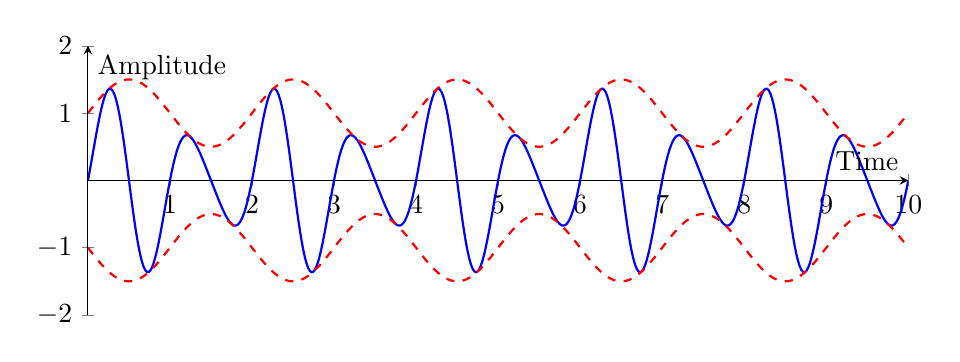
\begin{tikzpicture}
        \begin{axis}[
            width=12cm, height=5cm,
            xlabel={Time}, ylabel={Amplitude},
            axis lines=middle,
            xmin=0, xmax=10,
            ymin=-2, ymax=2,
            samples=500,
        ]
        % Normal modulation
        \addplot [blue, thick, domain=0:10] { (1 + 0.5*sin(deg(2*pi*x/2)))*sin(deg(2*pi*x)) };
        \addplot [red, thick, dashed, domain=0:10] { 1 + 0.5*sin(deg(2*pi*x/2)) };
        \addplot [red, thick, dashed, domain=0:10] { -1 - 0.5*sin(deg(2*pi*x/2)) };
        \end{axis}
    \end{tikzpicture}
    \caption{Normal Modulation ($m = 1$)}

    \vspace{1cm}

    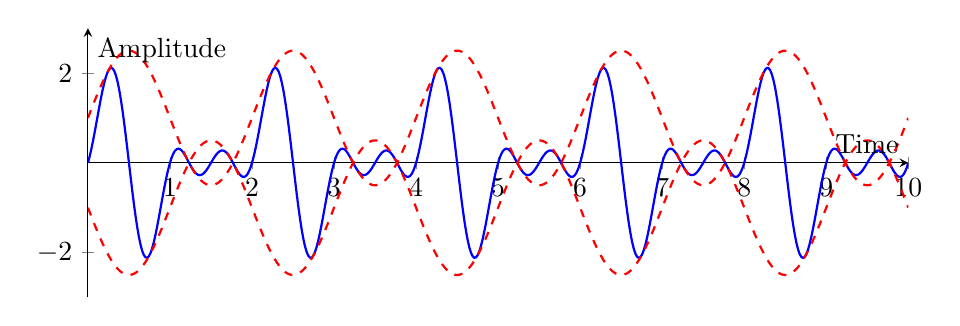
\begin{tikzpicture}
        \begin{axis}[
            width=12cm, height=5cm,
            xlabel={Time}, ylabel={Amplitude},
            axis lines=middle,
            xmin=0, xmax=10,
            ymin=-3, ymax=3,
            samples=500,
        ]
        % Over-modulation
        \addplot [blue, thick, domain=0:10] { (1 + 1.5*sin(deg(2*pi*x/2)))*sin(deg(2*pi*x)) };
        \addplot [red, thick, dashed, domain=0:10] { 1 + 1.5*sin(deg(2*pi*x/2)) };
        \addplot [red, thick, dashed, domain=0:10] { -1 - 1.5*sin(deg(2*pi*x/2)) };
        \end{axis}
    \end{tikzpicture}
    \caption{Over-Modulation ($m > 1$)}
%\caption{Illustrations of AM waveforms: Normal Modulation and Over-Modulation}
\end{figure}

  
\mybox{mygreen}{
    \textbf{Fun Fact}:  Modern technology has enabled hams to operate their station remotely from halfway around the world using Internet and radio links, adding new dimensions to amateur radio. But the fundamental rules related to transmission and interference still apply.
    }


\subsection*{Key Concepts for the Questions}
\begin{itemize}
    \item \textbf{Data emission:}  Digital signals used for transferring information.
    \item \textbf{Foreign Communications:} Transmissions sent to or received from amateur stations in other countries.
    \item \textbf{IARP:} International Amateur Radio Permit; enables operations in countries in Americas.
    \item \textbf{CEPT:} European Conference of Postal and Telecommunications administrations. Enables operations in most European countries.
    \item \textbf{Third Party Communications:} Passing messages on behalf of other people, not the operator.
    \item \textbf{Utilities Technology Council (UTC):} An organization that facilitates notification before operation on specific bands.
    \item \textbf{Angle modulation:} A type of modulation where the information is encoded in the phase or frequency.
    \item \textbf{Spurious emission:} Unwanted radio signals transmitted outside the desired bandwidth.
\end{itemize}

\subsection*{Practice Questions}
\begin{enumerate}
    \item What is the maximum bandwidth for a data emission on 60 meters?
        \begin{enumerate}
       \item 60 Hz
        \item  170 Hz
      \item  1.5 kHz
        \item \textbf {2.8 kHz}
    \end{enumerate}
     \textcolor{myred}{Explanation:}
     The FCC specifies the maximum bandwidth of 2.8 kHz for digital modes on the 60-meter band.
        
        \item Which of the following apply to communications transmitted to amateur stations in foreign countries?
    \begin{enumerate}
        \item Third party traffic must be limited to that intended for the exclusive use of government and non-Government Organization (NGOs) involved in emergency relief activities
        \item  All transmissions must be in English
        \item \textbf {Communications must be limited to those incidental to the purpose of the amateur service and remarks of a personal nature}
        \item  All these choices are correct
    \end{enumerate}
     \textcolor{myred}{Explanation:}
    Transmissions to stations in foreign countries must be non-commercial, non-political and limited to personal topics.
        
        \item How long must an operator wait after filing a notification with the Utilities Technology Council (UTC) before operating on the 2200-meter or 630-meter band?
        \begin{enumerate}
          \item Operators must not operate until approval is received
       \item \textbf {Operators may operate after 30 days, providing they have not been told that their station is within 1 kilometer of PLC systems using those frequencies}
      \item  Operators may not operate until a test signal has been transmitted in coordination with the local power company
    \item  Operations may commence immediately, and may continue unless interference is reported by the UTC
       \end{enumerate}
       \textcolor{myred}{Explanation:}
      Once the operator files a notification to UTC for operations in 2200m and 630m band, operation can commence after 30 days.
        
        \item What is an IARP?
       \begin{enumerate}
        \item \textbf {A permit that allows US amateurs to operate in certain countries of the Americas}
         \item  The internal amateur radio practices policy of the FCC
        \item  An indication of increased antenna reflected power
       \item  A forecast of intermittent aurora radio propagation
        \end{enumerate}
        \textcolor{myred}{Explanation:}
      IARP or International Amateur Radio Permit allows operations in select countries in Americas.

    \item Under what situation may a station transmit third party communications while being automatically controlled?
        \begin{enumerate}
        \item Never
          \item \textbf {Only when transmitting RTTY or data emissions}
         \item  Only when transmitting SSB or CW
        \item  On any mode approved by the National Telecommunication and Information Administration
     \end{enumerate}
       \textcolor{myred}{Explanation:}
        Third party communications can only be transmitted in data mode and under automatic control.

    \item Which of the following is required in order to operate in accordance with CEPT rules in foreign countries where permitted?
       \begin{enumerate}
         \item You must identify in the official language of the country in which you are operating
    \item  The US embassy must approve of your operation
    \item \textbf {You must have a copy of FCC Public Notice DA 16-1048}
        \item  You must append "/CEPT" to your call sign
    \end{enumerate}
        \textcolor{myred}{Explanation:}
     FCC public notice DA 16-1048 lists conditions of operations under CEPT.

     \item What notifications must be given before transmitting on the 630- or 2200-meter bands?
   \begin{enumerate}
         \item A special endorsement must be requested from the FCC
       \item  An environmental impact statement must be filed with the Department of the Interior
    \item  Operators must inform the FAA of their intent to operate, giving their call sign and distance to the nearest runway
      \item \textbf {Operators must inform the Utilities Technology Council (UTC) of their call sign and coordinates of the station}
    \end{enumerate}
        \textcolor{myred}{Explanation:}
         To start operations in 630m or 2200m band the operators must inform UTC about their call sign and coordinates.
      
        \item What is the maximum permissible duration of a remotely controlled station's transmissions if its control link malfunctions?
         \begin{enumerate}
         \item 30 seconds
        \item \textbf {3 minutes}
      \item  5 minutes
        \item  10 minutes
        \end{enumerate}
           \textcolor{myred}{Explanation:}
         If remote control malfunctions, the station can only transmit for maximum 3 minutes.
        
        \item What is the highest modulation index permitted at the highest modulation frequency for angle modulation below 29.0 MHz?
       \begin{enumerate}
        \item 0.5
        \item \textbf {1.0}
       \item  2.0
      \item  3.0
     \end{enumerate}
       \textcolor{myred}{Explanation:}
    The modulation index must be less than 1.0 for any angle modulation below 29 MHz.
        
       \item What is the maximum mean power level for a spurious emission below 30 MHz with respect to the fundamental emission?
        \begin{enumerate}
     \item \textbf {- 43 dB}
        \item  - 53 dB
       \item  - 63 dB
        \item  - 73 dB
    \end{enumerate}
   \textcolor{myred}{Explanation:}
    The power of a spurious emission below 30 MHz must be at least 43 dB less than fundamental power.
       
     \item Which of the following operating arrangements allows an FCC-licensed US citizen to operate in many European countries, and amateurs from many European countries to operate in the US?
      \begin{enumerate}
      \item \textbf {CEPT}
        \item  IARP
      \item  ITU reciprocal license
     \item  All these choices are correct
      \end{enumerate}
      \textcolor{myred}{Explanation:}
       CEPT allows reciprocal operations in many European countries as well as the US.

        \item In what portion of the 630-meter band are phone emissions permitted?
         \begin{enumerate}
          \item None
          \item  Only the top 3 kHz
           \item  Only the bottom 3 kHz
       \item \textbf {The entire band}
       \end{enumerate}
        \textcolor{myred}{Explanation:}
     Phone operation is permitted throughout the 630 meter band.
\end{enumerate}


% ------------------------------------------------------------------------
% SECTION E1D: Amateur Space and Earth Stations
% ------------------------------------------------------------------------
\section{E1D: Amateur Space and Earth Stations}
\subsection*{Understanding the Basics}
   \textcolor{myblue}{\textbf{Amateur space and earth stations}} are radio facilities for communicating through satellites and balloons that are more than 50 km above the Earth's surface. They have special rules regarding telemetry, telecommand, and identification.
\par
   \textcolor{myblue}{\textbf{Telemetry}} refers to the transmission of data or measurements to a ground station.
   \textcolor{myblue}{\textbf{Telecommand}} signals are used to remotely control the station. These communications follow specific rules in order to reduce interference with the other services and operations.
   \textcolor{myblue}{\textbf{One-way communications}} are usually prohibited but is allowed for beacons and space stations.

\mybox{mygreen}{
  \textbf{Fun Fact}: Some of the most exciting amateur radio activities occur through satellite communications. The International Space Station (ISS) often has amateur radio gear onboard that can be used to talk with astronauts! There are also a whole collection of small amateur satellites that you can contact.
  }


\subsection*{Key Concepts for the Questions}
\begin{itemize}
    \item \textbf{Telemetry:} The one way transmission of measurements.
        \item \textbf{Telecommand:} The signals that control a remote system.
    \item \textbf{Space Telecommand Station:} The earth station that sends telecommand signals to space.
    \item \textbf{One-way transmission:} Transmission from a station with no response from the receiving station.
     \item \textbf{Earth Station:} An amateur station that communicates with the space station.
      \item \textbf{HF/VHF/UHF Bands:} High frequency, very high frequency, and ultra high frequency amateur bands.
      \item \textbf{AMASAT:} Radio Amateur Satellite Corporation

\end{itemize}

\subsection*{Practice Questions}
\begin{enumerate}
  \item What is the definition of telemetry?
    \begin{enumerate}
        \item \textbf {One-way transmission of measurements at a distance from the measuring instrument}
        \item  Two-way transmissions in excess of 1000 feet
       \item  Two-way transmissions of data
        \item  One-way transmission that initiates, modifies, or terminates the functions of a device at a distance
    \end{enumerate}
    \textcolor{myred}{Explanation:}
    Telemetry is the transmission of data from a remote location for measurement. It is a one way communication.

    \item Which of the following may transmit encrypted messages?
     \begin{enumerate}
        \item Telecommand signals to terrestrial repeaters
        \item \textbf {Telecommand signals from a space telecommand station}
        \item  Auxiliary relay links carrying repeater audio
        \item  Mesh network backbone nodes
    \end{enumerate}
      \textcolor{myred}{Explanation:}
    Only space telecommand station may transmit encrypted messages.
    
    \item What is a space telecommand station?
    \begin{enumerate}
      \item An amateur station located on the surface of the Earth for communication with other Earth stations by means of Earth satellites
        \item \textbf {An amateur station that transmits communications to initiate, modify, or terminate functions of a space station}
     \item  An amateur station located in a satellite or a balloon more than 50 kilometers above the surface of the Earth
        \item  An amateur station that receives telemetry from a satellite or balloon more than 50 kilometers above the surface of the Earth
    \end{enumerate}
       \textcolor{myred}{Explanation:}
    A space telecommand station is a station on earth that sends telecommand to satellites and other space stations.

    \item Which of the following is required in the identification transmissions from a balloon-borne telemetry station?
       \begin{enumerate}
          \item \textbf {Call sign}
        \item  The output power of the balloon transmitter
        \item  The station's six-character Maidenhead grid locator
        \item  All these choices are correct
    \end{enumerate}
         \textcolor{myred}{Explanation:}
    A ballon-born telemetry station is required to identify by callsign at the beginning of the transmission.
    
        \item What must be posted at the location of a station being operated by telecommand on or within 50 kilometers of the Earth's surface?
      \begin{enumerate}
        \item A photocopy of the station license
        \item  A label with the name, address, and telephone number of the station licensee
    \item  A label with the name, address, and telephone number of the control operator
      \item \textbf {All these choices are correct}
    \end{enumerate}
          \textcolor{myred}{Explanation:}
     At a telecommand station, the station license, licensee information, and control operator information should be posted.
      
        \item What is the maximum permitted transmitter output power when operating a model craft by telecommand?
       \begin{enumerate}
         \item 1 watt
        \item \textbf {2 watts}
        \item  5 watts
        \item  100 watts
    \end{enumerate}
          \textcolor{myred}{Explanation:}
       The power limit for telecommand operation of a model craft is 2 watts.
       
    \item Which of the following HF amateur bands include allocations for space stations?
      \begin{enumerate}
    \item \textbf {40 meters, 20 meters, 15 meters, and 10 meters}
        \item  30 meters, 17 meters, and 10 meters
        \item  Only 10 meters
        \item  Satellite operation is permitted on all HF bands
    \end{enumerate}
       \textcolor{myred}{Explanation:}
    40, 20, 15, and 10 meter bands has allocations for space stations.

      \item Which VHF amateur bands have frequencies authorized for space stations?
        \begin{enumerate}
        \item 6 meters and 2 meters
       \item  6 meters, 2 meters, and 1.25 meters
         \item  2 meters and 1.25 meters
     \item \textbf {2 meters}
        \end{enumerate}
      \textcolor{myred}{Explanation:}
    2 meter band is among the most used VHF band for space operations.
         
    \item Which UHF amateur bands have frequencies authorized for space stations?
       \begin{enumerate}
      \item 70 centimeters only
       \item \textbf {70 centimeters and 13 centimeters}
    \item  70 centimeters and 33 centimeters
       \item  33 centimeters and 13 centimeters
     \end{enumerate}
     \textcolor{myred}{Explanation:}
        70cm and 13 cm band are among the most used UHF bands for space operations.
       
      \item Which amateur stations are eligible to be telecommand stations of space stations, subject to the privileges of the class of operator license held by the control operator of the station?
    \begin{enumerate}
        \item Any amateur station approved by AMSAT
        \item \textbf {Any amateur station so designated by the space station licensee}
       \item  Any amateur station so designated by the ITU
        \item  All these choices are correct
    \end{enumerate}
        \textcolor{myred}{Explanation:}
       A space station licensee can designate any amateur station for telecommand.
   
      \item Which amateur stations are eligible to operate as Earth stations?
      \begin{enumerate}
        \item Any amateur licensee who has successfully completed the AMSAT space communications course
      \item  Only those of General, Advanced or Amateur Extra class operators
       \item  Only those of Amateur Extra class operators
        \item \textbf {Any amateur station, subject to the privileges of the class of operator license held by the control operator}
     \end{enumerate}
      \textcolor{myred}{Explanation:}
    Any amateur station that complies with band and mode limits can be a ground station.
    
     \item Which of the following amateur stations may transmit one-way communications?
      \begin{enumerate}
        \item \textbf {A space station, beacon station, or telecommand station}
       \item  A local repeater or linked repeater station
       \item  A message forwarding station or automatically controlled digital station
        \item  All these choices are correct
        \end{enumerate}
         \textcolor{myred}{Explanation:}
       Space station, beacon, and telecommand stations are permitted one way transmissions
\end{enumerate}


% ------------------------------------------------------------------------
% SECTION E1F: Miscellaneous Rules
% ------------------------------------------------------------------------
\section{E1F: Miscellaneous Rules}

\subsection*{Understanding the Basics}
  \textcolor{myblue}{\textbf{Miscellaneous rules}} encompasses a range of topics including use of external RF amplifiers, prohibited communications, spread spectrum operation, auxiliary stations, operation of Canadian amateurs in the US, and special temporary authorities.
  \par
 \textcolor{myblue}{\textbf{External RF power amplifiers}} can enhance the power of a radio transmission. Rules for their design, sale, and use are set by FCC.
   \par
  \textcolor{myblue}{\textbf{Prohibited communications}} are also set by FCC, for example, transmissions for hire or material gain is usually prohibited.
  \par
  \textcolor{myblue}{\textbf{Spread spectrum}} is a transmission method using a much broader bandwidth that traditional modulation. It has special use conditions.
\par
    \textcolor{myblue}{\textbf{Special temporary authority (STA)}} is a special permission granted by FCC, to allow exceptions to the FCC rules for the reasons such as experiments or public service.
  
\mybox{mygreen}{
    \textbf{Fun Fact}:  The rules governing amateur radio have evolved over more than 100 years and are meant to balance experimentation with the need to prevent harmful interference.  This continues to evolve with the advance of technology and new operating practices.
    }

\subsection*{Key Concepts for the Questions}
\begin{itemize}
        \item \textbf{Spread Spectrum:} Transmission techniques that use a wider bandwidth than traditional modulation.
      \item \textbf{External RF power amplifiers:} Devices used to increase the transmitter power.
          \item \textbf{Auxiliary Station:} A station used for relaying or controlling other stations.
    \item \textbf{Special Temporary Authority (STA):} Permission by the FCC for a temporary deviation from standard rules.
    \item \textbf{Line A:} An imaginary line used to define geographic areas for special rules.
    \item \textbf{Pecuniary Interest:} Personal financial gain.
       \item \textbf{FCC certification:} Approval from FCC to operate devices in amateur bands.
\end{itemize}

\subsection*{Practice Questions}
\begin{enumerate}
    \item On what frequencies are spread spectrum transmissions permitted?
        \begin{enumerate}
        \item Only on amateur frequencies above 50 MHz
    \item \textbf {Only on amateur frequencies above 222 MHz}
      \item  Only on amateur frequencies above 420 MHz
        \item  Only on amateur frequencies above 144 MHz
    \end{enumerate}
     \textcolor{myred}{Explanation:}
        FCC allows spread spectrum on bands above 222 MHz.

     \item What privileges are authorized in the US to persons holding an amateur service license granted by the government of Canada?
     \begin{enumerate}
          \item None, they must obtain a US license
       \item  Full privileges of the General class license on the 80-, 40-, 20-, 15-, and 10-meter bands
       \item \textbf {The operating terms and conditions of the Canadian amateur service license, not to exceed US Amateur Extra class license privileges}
     \item  Full privileges, up to and including those of the Amateur Extra class license, on the 80-, 40-, 20-, 15-, and 10-meter bands
        \end{enumerate}
    \textcolor{myred}{Explanation:}
     Canadian operators with a reciprocal agreement may operate in the US, but not exceeding the same privileges granted to US extra-class license holder.
    
     \item Under what circumstances may a dealer sell an external RF power amplifier capable of operation below 144 MHz if it has not been granted FCC certification?
    \begin{enumerate}
    \item Gain is less than 23 dB when driven by power of 10 watts or less
    \item  The equipment dealer assembled it from a kit
   \item  It was manufactured and certificated in a country which has a reciprocal certification agreement with the FCC
      \item \textbf {The amplifier is constructed or modified by an amateur radio operator for use at an amateur station}
   \end{enumerate}
        \textcolor{myred}{Explanation:}
     If the amplifier was constructed or modified by an amateur operator for his/her station, the amplifier can be legally sold even without FCC certification.
     
      \item Which of the following geographic descriptions approximately describes "Line A"?
      \begin{enumerate}
     \item \textbf {A line roughly parallel to and south of the border between the US and Canada}
       \item  A line roughly parallel to and west of the US Atlantic coastline
   \item  A line roughly parallel to and north of the border between the US and Mexico
      \item  A line roughly parallel to and east of the US Pacific coastline
     \end{enumerate}
      \textcolor{myred}{Explanation:}
      Line A is an imaginary line roughly parallel to and south of the US-Canadian border.
        
    \item Amateur stations may not transmit in which of the following frequency segments if they are located in the contiguous 48 states and north of Line A?
    \begin{enumerate}
          \item 440 MHz - 450 MHz
         \item  53 MHz - 54 MHz
       \item  222 MHz - 223 MHz
      \item \textbf {420 MHz - 430 MHz}
    \end{enumerate}
   \textcolor{myred}{Explanation:}
    The 420 to 430 MHz band is a radio astronomy band and operation by amateur stations is prohibited in the area north of Line A.

    \item Under what circumstances might the FCC issue a Special Temporary Authority (STA) to an amateur station?
       \begin{enumerate}
       \item \textbf {To provide for experimental amateur communications}
      \item  To allow use of a special event call sign
   \item  To allow a VE group with less than three VEs to administer examinations in a remote, sparsely populated area
      \item  To allow a licensee who has passed an upgrade exam to operate with upgraded privileges while waiting for posting on the FCC database
      \end{enumerate}
       \textcolor{myred}{Explanation:}
    An STA may be granted to allow experimental communication that deviates from standard rules.
        
    \item When may an amateur station send a message to a business?
      \begin{enumerate}
        \item When the pecuniary interest of the amateur or his or her employer is less than \$25
          \item  When the pecuniary interest of the amateur or his or her employer is less than \$50
       \item  At no time
       \item \textbf {When neither the amateur nor their employer has a pecuniary interest in the communications}
        \end{enumerate}
    \textcolor{myred}{Explanation:}
      In general, messages with a pecuniary interest are prohibited unless the amateur or the employer does not have a financial interest in the communications.
       
       \item Which of the following types of amateur station communications are prohibited?
      \begin{enumerate}
        \item \textbf {Communications transmitted for hire or material compensation, except as otherwise provided in the rules}
      \item  Communications that have political content, except as allowed by the Fairness Doctrine
      \item  Communications that have religious content
     \item  Communications in a language other than English
        \end{enumerate}
    \textcolor{myred}{Explanation:}
     Amateur operation cannot be used for material gain, including compensation, unless specifically authorized by FCC regulations.
     
     \item Which of the following cannot be transmitted over an amateur radio mesh network?
      \begin{enumerate}
      \item Third party traffic
          \item  Email
       \item \textbf {Messages encoded to obscure their meaning}
       \item  All these choices are correct
      \end{enumerate}
      \textcolor{myred}{Explanation:}
      Encoding the message to obscure their content is prohibited in amateur bands.
       
      \item Who may be the control operator of an auxiliary station?
        \begin{enumerate}
          \item Any licensed amateur operator
          \item \textbf {Only Technician, General, Advanced, or Amateur Extra class operators}
        \item  Only General, Advanced, or Amateur Extra class operators
         \item  Only Amateur Extra class operators
        \end{enumerate}
     \textcolor{myred}{Explanation:}
       A technician or higher class licensee may be the control operator for an auxiliary station.
       
      \item Which of the following best describes one of the standards that must be met by an external RF power amplifier if it is to qualify for a grant of FCC certification?
         \begin{enumerate}
       \item It must produce full legal output when driven by not more than 5 watts of mean RF input power
      \item  It must have received an Underwriters Laboratory certification for electrical safety as well as having met IEEE standard 14.101(B)
        \item  It must exhibit a gain of less than 23 dB when driven by 10 watts or less
     \item \textbf {It must satisfy the FCC's spurious emission standards when operated at the lesser of 1500 watts or its full output power}
        \end{enumerate}
          \textcolor{myred}{Explanation:}
    An external RF amplifier must adhere to FCC's spurious emission standards when operated with an output power of 1.5KW, or full output power, which ever is less.
\end{enumerate}



\chapter{E2: Operating Procedures}


% ------------------------------------------------------------------------
% SECTION E2A: Amateur Radio in Space
% ------------------------------------------------------------------------
\section{E2A: Amateur Radio in Space - Reaching for the Stars!}

\subsection*{Understanding the Basics}
Get ready to launch into the exciting world of \textcolor{myblue}{\textbf{amateur radio in space}}! We’re talking about communicating through satellites, whether they're circling the Earth or zipping through the solar system. This area covers how ham operators use those wonderful tools in space.
\par
    You will get to know  \textcolor{myblue}{\textbf{Amateur Satellites}}, often known as "birds", these are our space based relays for communicating! Understanding the basics of \textcolor{myblue}{\textbf{Orbital Mechanics}} will make sure that you understand how the position of the satellites changes relative to Earth. This knowledge will give you a better chance to access these satellites when they're above your horizon.
\par
We'll also touch upon  \textcolor{myblue}{\textbf{Frequencies and Modes}} used for communication with satellites as well as \textcolor{myblue}{\textbf{satellite hardware}}, and \textcolor{myblue}{\textbf{satellite operations}}—the nitty-gritty of how to make contact!

\mybox{mygreen}{
  \textbf{Fun Fact}: Did you know that some satellites used by hams are designed, built and launched by amateurs? This is a remarkable demonstration of what a combined enthusiasm, ingenuity, and team work can create. There are plenty of resources available to learn and join these communities!
  }


\subsection{Inverting Linear Transponders}

An \textit{inverting linear transponder} is a specialized type of radio repeater, commonly employed in communication satellites, that reverses the frequency order of the received signals before re-transmission. This section details its operation and purpose.

\subsubsection*{Basic Function}

Unlike traditional repeaters that operate on a single frequency pair, a linear transponder handles a range, or band, of frequencies. Its core functionalities include:

\begin{itemize}
    \item \textbf{Receiving a frequency band:} The transponder receives a range of frequencies on the uplink (ground to satellite).
    \item \textbf{Frequency conversion:} This received band is shifted to a different frequency range for the downlink (satellite to ground). This frequency translation is essential to prevent interference between the uplink and downlink signals.
    \item \textbf{Frequency order inversion:} This is the defining characteristic of an inverting transponder. A signal received at the higher end of the uplink band is re-transmitted at the \textit{lower} end of the downlink band, and vice versa.
\end{itemize}

\subsubsection*{Mechanism of Inversion}

Frequency inversion is typically achieved through a \textit{mixer} circuit. A mixer combines two input frequencies, producing output signals at the sum and difference of these frequencies. In an inverting transponder:

\begin{enumerate}
    \item The received uplink signal is mixed with a locally generated frequency within the transponder.
    \item The \textit{difference} frequency resulting from this mixing process is selected for re-transmission. This selection of the difference frequency is what causes the frequency inversion.
\end{enumerate}

\textbf{Example:} Consider a transponder with an uplink band of 144–146 MHz and a downlink band of 435–437 MHz. If a signal is received at 145 MHz (mid-band) and mixed with a local oscillator frequency of 580 MHz, the difference frequency is $580 \, \text{MHz} - 145 \, \text{MHz} = 435 \, \text{MHz}$. However, a signal received at 146 MHz (high end of the uplink) results in a difference frequency of $580 \, \text{MHz} - 146 \, \text{MHz} = 434 \, \text{MHz}$. This demonstrates the inversion; a higher uplink frequency corresponds to a lower downlink frequency.

\subsubsection*{Rationale for Inversion: Doppler Mitigation}

The primary motivation for using inverting transponders, particularly in satellite communications, is to mitigate the \textit{Doppler effect}.

\begin{itemize}
    \item \textbf{Doppler effect:} The relative motion between a satellite and a ground station causes a frequency shift in the received signal. The frequency increases as the satellite approaches and decreases as it recedes.
    \item \textbf{Inverting transponders and Doppler:} The frequency inversion in the transponder effectively cancels out a significant portion of the Doppler shift. A positive Doppler shift on the uplink is largely counteracted by a negative Doppler shift on the downlink, simplifying tuning for ground stations.
\end{itemize}

\subsubsection*{Consequences of Inversion}

The frequency inversion has some important consequences:

\begin{itemize}
    \item \textbf{Sideband reversal:} Single-sideband (SSB) signals are inverted. Transmitting with upper sideband (USB) on the uplink will result in lower sideband (LSB) reception on the downlink, and vice versa.
    \item \textbf{Tuning considerations:} Operators must account for the frequency inversion when tuning their radios. Tuning "up" on the uplink necessitates tuning "down" on the downlink.
\end{itemize}

In conclusion, inverting linear transponders are crucial components in satellite communication systems, effectively mitigating the Doppler effect and facilitating reliable communication despite the relative motion between satellites and ground stations.


  
\subsection*{Key Concepts for the Questions}
\begin{itemize}
    \item \textbf{Ascending/Descending Pass:} The direction a satellite appears to be moving across the sky.
    \item \textbf{Linear Transponder:} A type of satellite repeater that re-transmits signals without demodulating and remodulating them.
    \item \textbf{Mode:} Describes the uplink and downlink frequency bands used by a satellite.
    \item \textbf{Keplerian Elements:}  Parameters defining the orbit of a satellite.
    \item \textbf{Circular Polarization:}  The method of transmission where the signal rotates as it transmits. This helps reduce the fading from signal reflections.
    \item \textbf{Effective Radiated Power (ERP):} Total power transmitted by antenna when considering the antenna gain. This limit is applied to many satellite operations.
     \item \textbf{Geostationary orbit:} The satellite is fixed at the same location on earth relative to ground.
    \item \textbf{L and S bands:} specific frequency bands commonly used in satellite communication.
    \item \textbf{Digital store-and-forward:} A mode of satellite operation which stores and transmits messages.

\end{itemize}

\subsection*{Practice Questions}
\begin{enumerate}
      \item What is the direction of an ascending pass for an amateur satellite?
    \begin{enumerate}
        \item  From west to east
       \item  From east to west
        \item \textbf{C. From south to north}
        \item  From north to south
    \end{enumerate}
    \textcolor{myred}{Explanation:}
    When a satellite is ascending, its path will appear to be moving from south towards north.
    
    \item Which of the following is characteristic of an inverting linear transponder?
       \begin{enumerate}
        \item  Doppler shift is reduced because the uplink and downlink shifts are in opposite directions
        \item  Signal position in the band is reversed
       \item  Upper sideband on the uplink becomes lower sideband on the downlink, and vice versa
        \item \textbf{D. All these choices are correct}
        \end{enumerate}
       \textcolor{myred}{Explanation:}
      In an inverting linear transponder, all of these behaviors happen to the signal.

     \item How is an upload signal processed by an inverting linear transponder?
     \begin{enumerate}
        \item  The signal is detected and remodulated on the reverse sideband
        \item  The signal is passed through a nonlinear filter
         \item  The signal is reduced to I and Q components, and the Q component is filtered out
        \item \textbf{D. The signal is mixed with a local oscillator signal and the difference product is transmitted}
        \end{enumerate}
    \textcolor{myred}{Explanation:}
    The signal is not demodulated, but simply mixed with a local oscillator for transmitting on different frequency.

    \item What is meant by the "mode" of an amateur radio satellite?
    \begin{enumerate}
    \item  Whether the satellite is in a low earth or geostationary orbit
        \item \textbf{B. The satellite's uplink and downlink frequency bands}
        \item  The satellite's orientation with respect to the Earth
       \item  Whether the satellite is in a polar or equatorial orbit
    \end{enumerate}
    \textcolor{myred}{Explanation:}
    The mode of a satellite refers to frequency ranges for uplink (receive) and downlink (transmit) for the satellite.
     
      \item What do the letters in a satellite's mode designator specify?
        \begin{enumerate}
        \item  Power limits for uplink and downlink transmissions
     \item  The location of the ground control station
         \item  The polarization of uplink and downlink signals
        \item \textbf{D. The uplink and downlink frequency ranges}
    \end{enumerate}
       \textcolor{myred}{Explanation:}
        Satellite designators specify the frequency ranges. For example "Mode VU" indicates a VHF uplink and UHF downlink.
       
        \item What are Keplerian elements?
        \begin{enumerate}
        \item \textbf{A. Parameters that define the orbit of a satellite}
        \item  Phase reversing elements in a Yagi antenna
    \item  High-emission heater filaments used in magnetron tubes
        \item  Encrypting codes used for spread spectrum modulation
    \end{enumerate}
        \textcolor{myred}{Explanation:}
        Keplerian elements are the parameters that define the orbit of any celestial objects.
    
        \item Which of the following types of signals can be relayed through a linear transponder?
        \begin{enumerate}
         \item  FM and CW
       \item  SSB and SSTV
       \item  PSK and packet
       \item \textbf{D. All these choices are correct}
        \end{enumerate}
    \textcolor{myred}{Explanation:}
     A linear transponder transmits all types of signal through.
      
         \item Why should effective radiated power (ERP) be limited to a satellite that uses a linear transponder?
    \begin{enumerate}
      \item  To prevent creating errors in the satellite telemetry
       \item \textbf{B. To avoid reducing the downlink power to all other users}
       \item  To prevent the satellite from emitting out-of-band signals
        \item  To avoid interfering with terrestrial QSOS
     \end{enumerate}
   \textcolor{myred}{Explanation:}
   Higher ERP in transponders, can saturate and cause reduction in transmitted power for other users.

   \item What do the terms "L band" and "S band" specify?
      \begin{enumerate}
      \item \textbf{A. The 23- and 13-centimeter bands}
        \item  The 2-meter and 70-centimeter bands
        \item  FM and digital store-and-forward systems
         \item  Which sideband to use
      \end{enumerate}
        \textcolor{myred}{Explanation:}
   L-Band and S-Band are among the many band designators. The specify a frequency range. L-band is roughly 23 cm wavelength and S band is around 13 cm wavelength.
         
          \item What type of satellite appears to stay in one position in the sky?
    \begin{enumerate}
        \item  HEO
         \item \textbf{B. Geostationary}
         \item  Geomagnetic
          \item  LEO
     \end{enumerate}
     \textcolor{myred}{Explanation:}
        A geostationary satellite appears in the same position due to the specific altitude and speed it circles earth, so that the orbit speed matches with Earth's rotation.

  \item What type of antenna can be used to minimize the effects of spin modulation and Faraday rotation?
        \begin{enumerate}
        \item  A linearly polarized antenna
      \item \textbf{B. A circularly polarized antenna}
        \item  An isotropic antenna
       \item  A log-periodic dipole array
     \end{enumerate}
       \textcolor{myred}{Explanation:}
        Circularly polarized antennas minimizes polarization problems of the received signals due to spin or Faraday rotation.
      
       \item What is the purpose of digital store-and-forward functions on an amateur radio satellite?
    \begin{enumerate}
     \item  To upload operational software for the transponder
     \item  To delay download of telemetry between satellites
      \item \textbf{C. To hold digital messages in the satellite for later download}
        \item  To relay messages between satellites
      \end{enumerate}
    \textcolor{myred}{Explanation:}
        Digital store-and-forward enables a satellite to store digital messages and send them later.
 
 \item Question Deleted (section not renumbered)
\end{enumerate}

% ------------------------------------------------------------------------
% SECTION E2B: Television Practices
% ------------------------------------------------------------------------
\section{E2B: Television Practices - Seeing is Believing!}

\subsection*{Understanding the Basics}
In this section, we'll be diving into the world of television through the lens of amateur radio. Get ready for concepts that are a bit different from audio communications.
We'll look at \textcolor{myblue}{\textbf{fast-scan television (FSTV) standards and techniques}}, which are used for high-resolution moving video signals, along with \textcolor{myblue}{\textbf{slow-scan television (SSTV) standards and techniques}}, a more resource-friendly way to send still images over radio. We will understand how images are created with these technologies.

\mybox{mygreen}{
  \textbf{Fun Fact}: Did you know that SSTV originated as a way to send images over the radio bands in the early 1900's?  It was designed to accommodate the limited bandwidth of radio channels at that time, using audio tones to represent different aspects of an image!
  }

\subsection*{Key Concepts for the Questions}
\begin{itemize}
    \item \textbf{Fast-Scan TV (FSTV):} A method to transmit high resolution, moving video.
    \item \textbf{Slow-Scan TV (SSTV):} A method of transmitting still images slowly over radio.
    \item \textbf{Interlaced Scanning:} A method of generating a picture by scanning alternating lines.
    \item \textbf{Vestigial Sideband Modulation:} A type of amplitude modulation where one sideband is mostly suppressed and another is transmitted.
    \item \textbf{Coding Rate:}  A parameter for forward error correction which relates the total data stream to the user information it carries.
      \item \textbf{DVB-T (Digital Video Broadcasting-Terrestrial):} A standard for digital TV transmission.
     \item \textbf{Digital Radio Mondiale (DRM):} A digital radio protocol, that can be used for transmitting slow scan tv signals.
         \item \textbf{Vertical Interval Signaling (VIS):} Control data sent with every slow-scan TV transmission.
\end{itemize}

\subsection*{Practice Questions}
\begin{enumerate}
    \item In digital television, what does a coding rate of 3/4 mean?
    \begin{enumerate}
       \item \textbf{A. 25\% of the data sent is forward error correction data}
        \item  Data compression reduces data rate by 3/4
       \item  1/4 of the time interval is used as a guard interval
       \item  Three, four-bit words are used to transmit each pixel
    \end{enumerate}
        \textcolor{myred}{Explanation:}
    A coding rate of 3/4, indicates 25% of the transmitted bits is used for error correction data.

  \item How many horizontal lines make up a fast-scan (NTSC) television frame?
      \begin{enumerate}
      \item  30
        \item  60
     \item \textbf{C. 525}
       \item  1080
    \end{enumerate}
    \textcolor{myred}{Explanation:}
     An NTSC frame consists of 525 horizontal lines.

  \item How is an interlaced scanning pattern generated in a fast-scan (NTSC) television system?
      \begin{enumerate}
        \item  By scanning two fields simultaneously
       \item  By scanning each field from bottom-to-top
     \item  By scanning lines from left-to-right in one field and right-to-left in the next
        \item \textbf{D. By scanning odd-numbered lines in one field and even-numbered lines in the next}
        \end{enumerate}
   \textcolor{myred}{Explanation:}
    In NTSC system, odd lines are drawn in first frame and even lines are drawn in second to generate a complete frame.

    \item How is color information sent in analog SSTV?
       \begin{enumerate}
        \item \textbf{A. Color lines are sent sequentially}
         \item  Color information is sent on a 2.8 kHz subcarrier
          \item  Color is sent in a color burst at the end of each line
         \item  Color is amplitude modulated on the frequency modulated intensity signal
        \end{enumerate}
    \textcolor{myred}{Explanation:}
    In analog SSTV, color is send as a series of sequential signals each carrying one primary color information.

       \item Which of the following describes the use of vestigial sideband in analog fast-scan TV transmissions?
    \begin{enumerate}
        \item  The vestigial sideband carries the audio information
      \item  The vestigial sideband contains chroma information
         \item \textbf{C. Vestigial sideband reduces the bandwidth while increasing the fidelity of low frequency video components}
       \item  Vestigial sideband provides high frequency emphasis to sharpen the picture
        \end{enumerate}
    \textcolor{myred}{Explanation:}
    The use of vestigial sideband modulation reduces the bandwith of the transmitted signal with minimal impact in the content.
    
    \item What is vestigial sideband modulation?
      \begin{enumerate}
       \item \textbf{A. Amplitude modulation in which one complete sideband and a portion of the other are transmitted}
         \item  A type of modulation in which one sideband is inverted
      \item  Narrow-band FM modulation achieved by filtering one sideband from the audio before frequency modulating the carrier
        \item  Spread spectrum modulation achieved by applying FM modulation following single sideband amplitude modulation
     \end{enumerate}
        \textcolor{myred}{Explanation:}
       In vestigial side band, one side band is transmitted completely and some parts of the other sideband is also included.

   \item Which types of modulation are used for amateur television DVB-T signals?
      \begin{enumerate}
          \item  FM and FSK
          \item \textbf{B. QAM and QPSK}
         \item  AM and OOK
         \item  All these choices are correct
        \end{enumerate}
       \textcolor{myred}{Explanation:}
     DVB-T signals typically use QAM and QPSK modulation for their transmissions.
     
    \item What technique allows commercial analog TV receivers to be used for fast-scan TV operations on the 70-centimeter band?
       \begin{enumerate}
      \item \textbf{A. Transmitting on channels shared with cable TV}
        \item  Using converted satellite TV dishes
         \item  Transmitting on the abandoned TV channel 2
      \item  Using USB and demodulating the signal with a computer sound card
        \end{enumerate}
      \textcolor{myred}{Explanation:}
        Many amateur transmissions utilize unused cable TV frequencies to be received on TV receivers.
      
     \item What kind of receiver can be used to receive and decode SSTV using the Digital Radio Mondiale (DRM) protocol?
      \begin{enumerate}
       \item  CDMA
       \item  AREDN
      \item  AM
       \item \textbf{D. SSB}
      \end{enumerate}
       \textcolor{myred}{Explanation:}
        DRM protocol used for slow-scan tv is modulated in SSB.

    \item What aspect of an analog slow-scan television signal encodes the brightness of the picture?
      \begin{enumerate}
      \item \textbf{A. Tone frequency}
        \item  Tone amplitude
    \item  Sync amplitude
       \item  Sync frequency
        \end{enumerate}
       \textcolor{myred}{Explanation:}
        In analog SSTV systems, image brightness is encoded as variation in the frequency of an audio signal.

         \item What is the function of the vertical interval signaling (VIS) code sent as part of an SSTV transmission?
       \begin{enumerate}
          \item  To lock the color burst oscillator in color SSTV images
        \item \textbf{B. To identify the SSTV mode being used}
       \item  To provide vertical synchronization
        \item  To identify the call sign of the station transmitting
        \end{enumerate}
       \textcolor{myred}{Explanation:}
        VIS code specifies the mode used for SSTV transmission.

    \item What signals SSTV receiving software to begin a new picture line?
    \begin{enumerate}
      \item \textbf{A. Specific tone frequencies}
       \item  Elapsed time
     \item  Specific tone amplitudes
       \item  A two-tone signal
    \end{enumerate}
    \textcolor{myred}{Explanation:}
       Specific tone frequencies indicate a new line beginning to the software.
\end{enumerate}



Okay, here's the LaTeX source code for sections E2C and E2D, continuing the previous structure and maintaining the cheerful tone!

% ------------------------------------------------------------------------
% SECTION E2C: Contest and DX Operating
% ------------------------------------------------------------------------
\section{E2C: Contest and DX Operating - Time to Compete and Explore!}

\subsection*{Understanding the Basics}
Get ready to ramp up the excitement with \textcolor{myblue}{\textbf{contest and DX operating}}! This is where the friendly competition and long-distance communication challenges meet. You will explore how to make contacts with rare stations using techniques and special skills.
We will learn about \textcolor{myblue}{\textbf{Remote operation techniques}} that allow you to control a radio station from a distance, making you a "contester" wherever you are.
Understanding how data is stored in a log is essential in \textcolor{myblue}{\textbf{log data formats}} and it is needed for contest submissions and DX contact confirmations. You will also explore the concept of \textcolor{myblue}{\textbf{contact confirmation}} and finally we will touch on the area of \textcolor{myblue}{\textbf{RF network systems}}, such as mesh networks.

\mybox{mygreen}{
  \textbf{Fun Fact}: Did you know some contesters work to set records for the total number of contacts during a given period of time?  Contests also foster innovative strategies that drive the development of new hardware and techniques in ham radio!
  }

\subsection*{Key Concepts for the Questions}
\begin{itemize}
    \item \textbf{Remote control/operation:} Operating a station from a distant location.
    \item \textbf{Contesting:}  Friendly competition of making the highest number of contacts in limited time.
     \item \textbf{Cabrillo Format:} A standard for submitting electronic contest logs.
     \item \textbf{Logbook of the World (LoTW):} An online service for confirming contacts with another operator.
    \item \textbf{DX QSL Manager:} Someone who handles incoming and outgoing QSL cards (contact confirmations) for a rare station.
    \item \textbf{National Calling Frequency:}  A common frequency used to initiate contact in different bands.
     \item \textbf{Mesh Networks:} A type of network that utilizes radio links for connecting devices over a large area.
    \item  \textbf{Latency:} The delay between an action and the corresponding change in transmitted signal

\end{itemize}

\subsection*{Practice Questions}
\begin{enumerate}
  \item What indicator is required to be used by US-licensed operators when operating a station via remote control and the remote transmitter is located in the US?
    \begin{enumerate}
        \item  / followed by the USPS two-letter abbreviation for the state in which the remote station is located
        \item  /R\# where \# is the district of the remote station
        \item  / followed by the ARRL Section of the remote station
        \item \textbf{D. No additional indicator is required}
    \end{enumerate}
     \textcolor{myred}{Explanation:}
     When the transmitter location and operation is within US territories, no specific location indicator is needed for a remotely controlled station.

  \item Which of the following file formats is used for exchanging amateur radio log data?
      \begin{enumerate}
      \item  NEC
        \item  ARLD
        \item \textbf{C. ADIF}
       \item  OCF
    \end{enumerate}
        \textcolor{myred}{Explanation:}
        ADIF is a standard for Amateur Data Interchange Format.
  
   \item From which of the following bands is amateur radio contesting generally excluded?
       \begin{enumerate}
       \item \textbf{A. 30 meters}
          \item  6 meters
        \item  70 centimeters
        \item  33 centimeters
    \end{enumerate}
      \textcolor{myred}{Explanation:}
    Contesting is not allowed on the 30 meter band.

    \item Which of the following frequencies can be used for amateur radio mesh networks?
        \begin{enumerate}
         \item  HF frequencies where digital communications are permitted
        \item \textbf{B. Frequencies shared with various unlicensed wireless data services}
     \item  Cable TV channels 41-43
       \item  The 60-meter band channel centered on 5373 kHz
     \end{enumerate}
        \textcolor{myred}{Explanation:}
     Many amateur mesh networks use frequencies allocated to unlicensed wireless services.

    \item What is the function of a DX QSL Manager?
        \begin{enumerate}
           \item  Allocate frequencies for DXpeditions
           \item \textbf{B. Handle the receiving and sending of confirmations for a DX station}
       \item  Run a net to allow many stations to contact a rare DX station
         \item  Communicate to a DXpedition about propagation, band openings, pileup conditions, etc.
       \end{enumerate}
        \textcolor{myred}{Explanation:}
     A QSL manager helps rare and DX stations with their contact confirmations, commonly referred as QSL cards.

   \item During a VHF/UHF contest, in which band segment would you expect to find the highest level of SSB or CW activity?
       \begin{enumerate}
     \item  At the top of each band, usually in a segment reserved for contests
      \item  In the middle of each band, usually on the national calling frequency
     \item \textbf{C. In the weak signal segment of the band, with most of the activity near the calling frequency}
     \item  In the middle of the band, usually 25 kHz above the national calling frequency
        \end{enumerate}
      \textcolor{myred}{Explanation:}
        The weak signal segment of VHF and UHF bands is typically reserved for contact with CW and SSB signals.

     \item What is the Cabrillo format?
       \begin{enumerate}
    \item \textbf{A. A standard for submission of electronic contest logs}
      \item  A method of exchanging information during a contest QSO
    \item  The most common set of contest rules
    \item  A digital protocol specifically designed for rapid contest exchanges
       \end{enumerate}
          \textcolor{myred}{Explanation:}
          Cabrillo is a standard file format used for exchanging contact log information in contesting events.
         
      \item Which of the following contacts may be confirmed through the Logbook of The World (LoTW)?
          \begin{enumerate}
      \item  Special event contacts between stations in the US
        \item  Contacts between a US station and a non-US station
         \item  Contacts for Worked All States credit
       \item \textbf{D. All these choices are correct}
    \end{enumerate}
         \textcolor{myred}{Explanation:}
      LoTW or Logbook of the world is an online system for all types of contact confirmation.

    \item What type of equipment is commonly used to implement an amateur radio mesh network?
       \begin{enumerate}
        \item  A 2-meter VHF transceiver with a 1,200-baud modem
         \item  A computer running EchoLink to provide interface from the radio to the internet
      \item \textbf{C. A wireless router running custom firmware}
     \item  A 440 MHz transceiver with a 9,600-baud modem
    \end{enumerate}
        \textcolor{myred}{Explanation:}
    Mesh networks generally utilize commercial wifi routers with specific firmwares to establish radio links.
     
      \item Why do DX stations often transmit and receive on different frequencies?
        \begin{enumerate}
     \item  Because the DX station may be transmitting on a frequency that is prohibited to some responding stations
         \item  To separate the calling stations from the DX station
    \item  To improve operating efficiency by reducing interference
      \item \textbf{D. All these choices are correct}
       \end{enumerate}
     \textcolor{myred}{Explanation:}
     A split frequency helps with interference, different rules of operation and keeps calling station out of the transmitting band.

   \item How should you generally identify your station when attempting to contact a DX station during a contest or in a pileup?
    \begin{enumerate}
    \item \textbf{A. Send your full call sign once or twice}
    \item  Send only the last two letters of your call sign until you make contact
  \item  Send your full call sign and grid square
  \item  Send the call sign of the DX station three times, the words “this is,” then your call sign three times
      \end{enumerate}
   \textcolor{myred}{Explanation:}
    When contacting a DX or contest station, you should keep identification short to avoid unnecessary traffic.

       \item What indicates the delay between a control operator action and the corresponding change in the transmitted signal?
    \begin{enumerate}
    \item  Jitter
      \item  Hang time
        \item \textbf{C. Latency}
      \item  Anti-VOX
        \end{enumerate}
        \textcolor{myred}{Explanation:}
    Latency is the name given to the time delay in a control system.
\end{enumerate}


\subsection{Amateur Data Interchange Format (ADIF)}

The Amateur Data Interchange Format (ADIF) is a standard file format used by amateur radio operators to exchange contact log information. It provides a structured and consistent way to store and share data about radio contacts (QSOs), making it easy to import and export logs between different logging software applications. This section describes the ADIF format and its key features.

\subsubsection{Purpose and Structure}

ADIF aims to standardize the exchange of QSO data, eliminating the need for manual conversion between different logging programs. Its structure is based on \textit{tags} and \textit{values}, similar to HTML or XML. Each QSO is represented as a set of tags, where each tag represents a specific piece of information about the contact, such as the callsign of the other station, the date and time of the contact, the frequency used, and the mode of operation.

A typical ADIF record for a single QSO looks like this (simplified example):

\begin{verbatim}
<CALL:6>W1AW
<QSO_DATE:8>20240426
<TIME_ON:4>1234
<BAND:3>20M
<MODE:2>CW
<EOR>
\end{verbatim}

\begin{itemize}
    \item \texttt{<TAG:length>} represents the tag name and the length of the associated value. For example, \texttt{<CALL:6>} indicates the tag is \texttt{CALL} and the value is 6 characters long.
    \item The value follows the tag.
    \item \texttt{<EOR>} (End of Record) marks the end of a single QSO record.
\end{itemize}

\subsubsection{Key Tags and Data Types}

ADIF defines a wide range of tags to capture various aspects of a QSO. Some of the most commonly used tags include:

\begin{itemize}
    \item \texttt{CALL}: The callsign of the contacted station.
    \item \texttt{QSO\_DATE}: The date of the QSO in YYYYMMDD format.
    \item \texttt{TIME\_ON}: The start time of the QSO in HHMM format (UTC).
    \item \texttt{BAND}: The frequency band used (e.g., 20M, 40M).
    \item \texttt{MODE}: The mode of operation (e.g., CW, SSB, FM).
    \item \texttt{RST\_SENT}: The signal report sent to the other station.
    \item \texttt{RST\_RCVD}: The signal report received from the other station.
    \item \texttt{NAME}: The name of the operator.
    \item \texttt{QTH}: The location of the station.
    \item \texttt{COUNTRY}: The country of the station.
\end{itemize}

ADIF supports various data types, including strings, integers, dates, and times, ensuring data integrity and consistency.

\subsubsection{ADIF Versions and Extensions}

Over time, ADIF has evolved to include new tags and features. Different versions of ADIF exist, and logging software usually supports a range of versions. Additionally, some software applications may use custom tags (known as \textit{user-defined fields} or UDFs) to store information not covered by the standard ADIF tags. These UDFs are prefixed with \texttt{USERDEF} and are useful for storing application-specific data.

\subsubsection{Benefits of Using ADIF}

Using ADIF provides numerous benefits for amateur radio operators:

\begin{itemize}
    \item \textbf{Interoperability:} It allows seamless exchange of log data between different logging programs.
    \item \textbf{Data preservation:} It provides a standardized format for archiving QSO data.
    \item \textbf{Log checking and analysis:} It facilitates log checking for awards and contests.
    \item \textbf{Online log submission:} Many online log submission systems for contests and awards accept ADIF files.
\end{itemize}

In summary, ADIF is an essential tool for modern amateur radio logging, enabling efficient data management and exchange within the amateur radio community.




% ------------------------------------------------------------------------
% SECTION E2D: Operating Methods: Digital Modes for VHF and UHF
% ------------------------------------------------------------------------
\section{E2D: Operating Methods: Digital Modes and Procedures for VHF and UHF - Digital Delights!}
\subsection*{Understanding the Basics}
This section is about exploring \textcolor{myblue}{\textbf{digital modes}} for VHF and UHF communication, where you will learn the magic of transmitting data across radio links using a wide variety of different techniques.
\par
   You will learn more about specialized digital modes for specific applications, such as  \textcolor{myblue}{\textbf{meteor scatter communications}} that bounces signals off of ionized trails of meteors. Then you will learn about \textcolor{myblue}{\textbf{APRS (Automatic Packet Reporting System)}} ,  a real time digital communication method for sending and receiving location data as well as text messages, and finally \textcolor{myblue}{\textbf{EME (Earth-Moon-Earth)} or moonbounce} which bounces radio signals off of the moon for longer distance contacts.

\mybox{mygreen}{
    \textbf{Fun Fact}: Many digital modes for VHF and UHF communications were created by hams who were looking for ways to expand the possibilities of digital radio. Ham radio continues to be an area where creativity and ingenuity drives the innovation.
  }

\subsection*{Key Concepts for the Questions}
\begin{itemize}
    \item \textbf{Meteor Scatter:} A technique for using radio signals bounced off of meteor trails to establish communication.
     \item \textbf{MSK144:} A specific digital mode designed for meteor scatter communication.
     \item \textbf{RST Report:} A code sent with radio transmissions to signify signal report.
    \item \textbf{Earth-Moon-Earth (EME):} Communication via bouncing signals off the Moon.
    \item \textbf{APRS (Automatic Packet Reporting System):} A digital system for real time location and data exchange.
    \item \textbf{JT65/FT8/FT4:} Digital modes designed for weak signal operation.
    \item  \textbf{ACK/NAK:} Packet communication signal for acknowledgements and lack of acknowledgement.
     \item \textbf{Digipeater:} A station that receives, temporarily stores and retransmits APRS data.
\end{itemize}

\subsection*{Practice Questions}
\begin{enumerate}
     \item Which of the following digital modes is designed for meteor scatter communications?
    \begin{enumerate}
     \item  WSPR
         \item \textbf{B. MSK144}
          \item  Hellschreiber
         \item  APRS
        \end{enumerate}
    \textcolor{myred}{Explanation:}
        MSK144 or Minimum Shift Keying (MSK), a type of Frequency Shift Keying is specifically used for meteor scatter communications.
     
    \item What information replaces signal-to-noise ratio when using the FT8 or FT4 modes in a VHF contest?
        \begin{enumerate}
           \item  RST report
       \item  State abbreviation
         \item  Serial number
        \item \textbf{D. Grid square}
    \end{enumerate}
       \textcolor{myred}{Explanation:}
     FT8/FT4 signals typically report the location of transmission, which is commonly expressed by a grid square instead of the traditional RST report.
       
      \item Which of the following digital modes is designed for EME communications?
     \begin{enumerate}
    \item  MSK144
         \item  PACTOR III
     \item  WSPR
      \item \textbf{D. Q65}
     \end{enumerate}
      \textcolor{myred}{Explanation:}
   Q65 digital mode was specifically designed to communicate for EME operation where signal to noise ratio is typically very low.
     
     \item What technology is used for real-time tracking of balloons carrying amateur radio transmitters?
      \begin{enumerate}
      \item  FT8
       \item  Bandwidth compressed LORAN
       \item \textbf{C. APRS}
        \item  PACTOR III
        \end{enumerate}
   \textcolor{myred}{Explanation:}
    APRS or Automatic Packet Reporting System is a common technology for tracking high-altitude balloons.

       \item What is the characteristic of the JT65 mode?
      \begin{enumerate}
     \item  Uses only a 65 Hz bandwidth
        \item \textbf{B. Decodes signals with a very low signal-to-noise ratio}
       \item  Symbol rate is 65 baud
         \item  Permits fast-scan TV transmissions over narrow bandwidth
        \end{enumerate}
     \textcolor{myred}{Explanation:}
        JT65 is famous for its capability for receiving weak signal, that is well under the typical noise floor.

    \item Which of the following is a method for establishing EME contacts?
     \begin{enumerate}
       \item \textbf{A. Time-synchronous transmissions alternating between stations}
         \item  Storing and forwarding digital messages
        \item  Judging optimum transmission times by monitoring beacons reflected from the moon
        \item  High-speed CW identification to avoid fading
     \end{enumerate}
     \textcolor{myred}{Explanation:}
     Due to extreme weak signal and timing issues, EME communication often involve a schedule alternating transmission times.

     \item What digital protocol is used by APRS?
         \begin{enumerate}
       \item  PACTOR
        \item  QAM
      \item \textbf{C. AX.25}
       \item  AMTOR
       \end{enumerate}
    \textcolor{myred}{Explanation:}
     APRS uses the AX.25 packet radio protocol for transferring messages.
   
    \item What type of packet frame is used to transmit APRS beacon data?
    \begin{enumerate}
     \item  Acknowledgement
     \item  Burst
   \item \textbf{C. Unnumbered Information}
         \item  Connect
      \end{enumerate}
     \textcolor{myred}{Explanation:}
     The beacon data in APRS is transmitted as Unnumbered Information (UI) frame.
       
     \item What type of modulation is used by JT65?
      \begin{enumerate}
        \item \textbf{A. Multitone AFSK}
         \item  PSK
       \item  RTTY
       \item  QAM
       \end{enumerate}
     \textcolor{myred}{Explanation:}
         JT65 mode uses Multitone Audio Frequency Shift Keying for encoding and decoding data.
        
     \item What does the packet path WIDE3-1 designate?
      \begin{enumerate}
      \item  Three stations are allowed on frequency, one transmitting at a time
      \item  Three subcarriers are permitted, subcarrier one is being used
       \item \textbf{C. Three digipeater hops are requested with one remaining}
        \item  Three internet gateway stations may receive one transmission
      \end{enumerate}
     \textcolor{myred}{Explanation:}
       WIDE3-1 directs a packet to be passed by three digipeaters, allowing one more hop from final digipeater.
     
    \item How do APRS stations relay data?
      \begin{enumerate}
      \item  By packet ACK/NAK relay
        \item \textbf{B. By C4FM repeaters}
       \item  By DMR repeaters
       \item  By packet digipeaters
      \end{enumerate}
    \textcolor{myred}{Explanation:}
      APRS data is commonly repeated through digipeaters using C4FM digital voice modulations.
\end{enumerate}

\section{E2E: Operating Methods: Digital Modes and Procedures for HF - Exploring HF Digital!}
\subsection*{Understanding the Basics}
Now, let's dive into the amazing world of \textcolor{myblue}{\textbf{digital modes on HF}}! This section is about how to use your radio to send digital data for longer distances through the atmosphere. You will discover the techniques used for those exciting contacts, using a variety of modulation schemes.
\par
    This section covers both the use of digital modes and the techniques and operation associated with the \textcolor{myblue}{\textbf{digital operation}}. You'll become familiar with everything needed for HF digital communication.

\mybox{mygreen}{
    \textbf{Fun Fact}:  Some digital modes for HF communication allow for contacts with signal power as low as a few milliwatts! These modes allow us to communicate globally, even with very modest station setups, truly showcasing the ingenuity of digital communication.
  }

\subsection*{Key Concepts for the Questions}
\begin{itemize}
      \item \textbf{FSK (Frequency Shift Keying):} A type of digital modulation where the frequency represents digital information.
        \item \textbf{WSJT-X:} A suite of software for weak signal communications using many digital modes.
      \item \textbf{FT4/FT8:} Digital modes optimized for weak signals and fast exchanges of brief messages.
      \item \textbf{PACTOR:} A sophisticated digital mode used for reliable data transfers under challenging conditions.
       \item  \textbf{RTTY (Radio Teletype):} A legacy digital mode.
    \item \textbf{MFSK16:} A multitone FSK modulation scheme.
    \item \textbf{AMTOR:} Amateur Teleprinting Over Radio, an early digital mode.
   \item \textbf{Direct FSK/Audio FSK:} Two different implementations of Frequency Shift Keying.
    
\end{itemize}

\subsection*{Practice Questions}
\begin{enumerate}
   \item Which of the following types of modulation is used for data emissions below 30 MHz?
    \begin{enumerate}
        \item  DTMF tones modulating an FM signal
        \item \textbf{B. FSK}
        \item  Pulse modulation
        \item  Spread spectrum
    \end{enumerate}
    \textcolor{myred}{Explanation:}
   Frequency shift keying is a very popular method of data encoding for transmission below 30 MHz.
       
    \item Which of the following synchronizes WSJT-X digital mode transmit/receive timing?
    \begin{enumerate}
        \item  Alignment of frequency shifts
        \item \textbf{B. Synchronization of computer clocks}
       \item  Sync-field transmission
        \item  Sync-pulse timing
    \end{enumerate}
    \textcolor{myred}{Explanation:}
        The synchronization of WSJT-X timing is entirely dependent on computer clock time.
        
    \item To what does the "4" in FT4 refer?
    \begin{enumerate}
        \item  Multiples of 4 bits of user information
        \item \textbf{B. Four-tone continuous-phase frequency shift keying}
        \item  Four transmit/receive cycles per minute
         \item  All these choices are correct
    \end{enumerate}
    \textcolor{myred}{Explanation:}
     FT4 uses 4 tones FSK modulation as its encoding scheme.
        
        \item Which of the following is characteristic of the FST4 mode?
      \begin{enumerate}
         \item  Four-tone Gaussian frequency shift keying
        \item  Variable transmit/receive periods
         \item  Seven different tone spacings
       \item \textbf{D. All these choices are correct}
        \end{enumerate}
    \textcolor{myred}{Explanation:}
     FST4 uses four tones with Gausian shaping. It also has variable transmit/receive periods. Finally, it uses 7 tone frequencies.

        \item Which of these digital modes does not support keyboard-to-keyboard operation?
    \begin{enumerate}
        \item \textbf{A. WSPR}
        \item  RTTY
        \item  PSK31
         \item  MFSK16
        \end{enumerate}
        \textcolor{myred}{Explanation:}
     WSPR or Weak Signal Propagation Reporter is a mode that is typically sent automatically with computer software, and not designed for keyboard operations.
         
        \item What is the length of an FT8 transmission cycle?
       \begin{enumerate}
      \item  It varies with the amount of data
        \item  8 seconds
      \item \textbf{C. 15 seconds}
         \item  30 seconds
        \end{enumerate}
   \textcolor{myred}{Explanation:}
    The typical transmission cycle of FT8 is fixed at 15 seconds.

   \item How does Q65 differ from JT65?
        \begin{enumerate}
        \item  Keyboard-to keyboard operation is supported
        \item  Quadrature modulation is used
        \item \textbf{C. Multiple receive cycles are averaged}
        \item  All these choices are correct
    \end{enumerate}
       \textcolor{myred}{Explanation:}
    Unlike JT65, Q65 mode will repeat many receive cycles to make the weak signal more robust to decode.

   \item Which of the following HF digital modes can be used to transfer binary files?
     \begin{enumerate}
        \item  PSK31
       \item \textbf{B. PACTOR}
         \item  RTTY
        \item  AMTOR
    \end{enumerate}
     \textcolor{myred}{Explanation:}
     PACTOR can transmit binary files along with other data.
       
        \item Which of the following HF digital modes uses variable-length character coding?
     \begin{enumerate}
       \item  RTTY
        \item  PACTOR
      \item  MT63
        \item \textbf{D. PSK31}
        \end{enumerate}
      \textcolor{myred}{Explanation:}
        PSK31 utilizes variable-length character coding which encodes most common characters with a shorter symbol sequence, thus requiring smaller bandwidth.
     
    \item Which of these digital modes has the narrowest bandwidth?
       \begin{enumerate}
       \item  MFSK16
         \item  170 Hz shift, 45-baud RTTY
         \item \textbf{C. FT8}
         \item  PACTOR IV
       \end{enumerate}
        \textcolor{myred}{Explanation:}
      FT8 signal has very narrow bandwidth due to its use of 70Hz tones and short transmission bursts.
        
    \item What is the difference between direct FSK and audio FSK?
       \begin{enumerate}
         \item \textbf{A. Direct FSK modulates the transmitter VFO}
      \item  Direct FSK occupies less bandwidth
      \item  Direct FSK can transmit higher baud rates
      \item  All these choices are correct
     \end{enumerate}
         \textcolor{myred}{Explanation:}
       Direct FSK directly manipulates the oscillator frequency while audio FSK applies FSK modulation in the audio stage before transmitter modulation.
        
        \item How do ALE stations establish contact?
         \begin{enumerate}
         \item \textbf{A. ALE constantly scans a list of frequencies, activating the radio when the designated call sign is received}
      \item  ALE radios monitor an internet site for the frequency they are being paged on
       \item  ALE radios send a constant tone code to establish a frequency for future use
        \item  ALE radios activate when they hear their signal echoed by back scatter
      \end{enumerate}
    \textcolor{myred}{Explanation:}
     ALE capable radios constantly scan designated frequencies, listening for a matching call sign.

      \item Which of these digital modes has the highest data throughput under clear communication conditions?
       \begin{enumerate}
        \item  MFSK16
        \item  170 Hz shift, 45 baud RTTY
        \item  FT8
        \item \textbf{D. PACTOR IV}
       \end{enumerate}
        \textcolor{myred}{Explanation:}
         PACTOR IV is a data mode that provides the highest through output when there are minimal interference and noise.
\end{enumerate}

%
% ************************************************************************
% CHAPTER 3: Sublement E3 - Radio Wave Propagation
% ************************************************************************
\chapter{E3: Radio Wave Propagation - Riding the Radio Waves!}

% ------------------------------------------------------------------------
% SECTION E3A: Electromagnetic Waves and Specialized Propagation
% ------------------------------------------------------------------------
\section{E3A: Electromagnetic Waves and Specialized Propagation - Where Do Radio Signals Go?}

\subsection*{Understanding the Basics}
Ready to understand what really happens when your radio signals leave your antenna? Get ready to take a journey through the fascinating world of \textcolor{myblue}{\textbf{electromagnetic waves and propagation}}! This section goes into several different methods of long and short range communications.
We'll delve into the specifics of \textcolor{myblue}{\textbf{Earth-Moon-Earth (EME) communications}}, a challenging yet awesome way of communicating through the moon. Then we will explore \textcolor{myblue}{\textbf{meteor scatter}}, that allows communication using meteor trails. Other modes such as \textcolor{myblue}{\textbf{tropospheric and scatter propagation}}, and \textcolor{myblue}{\textbf{auroral propagation}} also will be covered. Finally we will discuss \textcolor{myblue}{\textbf{daily variation of ionospheric propagation}} and the important topic of \textcolor{myblue}{\textbf{circular polarization}}.
\mybox{mygreen}{
  \textbf{Fun Fact}: Did you know that the ionosphere, a layer of Earth's atmosphere, is a major part of how radio waves travel across the globe?  It is an area of electrical activity that changes based on time of day, season and solar activity!
  }
\subsection*{Key Concepts for the Questions}
\begin{itemize}
    \item \textbf{Earth-Moon-Earth (EME):} Communication via bouncing signals off the Moon.
    \item \textbf{Meteor Scatter:} A communication technique that uses ionized trails of meteors to reflect signals.
    \item \textbf{Tropospheric Ducting:} The propagation of signals within atmospheric layers, that act as a duct to guide the signals over long distances.
        \item \textbf{Auroral Propagation:} A technique that uses reflections of signals off of the auroras for propagation.
        \item \textbf{Ionospheric Propagation:} Radio signals that are reflected by the ionosphere.
    \item \textbf{Libration Fading:} A type of fading specific to EME communication due to the moon's motion.
     \item \textbf{Perigee:} When moon is closest to the earth in its orbit.
         \item \textbf{Apogee:} When moon is farthest from the earth in its orbit.
        \item \textbf{MUF (Maximum Usable Frequency):} The highest frequency that can be used for ionospheric propagation.
        \item \textbf{Circular Polarization:} Signals with a rotating electric and magnetic field.

\end{itemize}

\subsection*{Practice Questions}
\begin{enumerate}
      \item What is the approximate maximum separation measured along the surface of the Earth between two stations communicating by EME?
       \begin{enumerate}
        \item  2,000 miles, if the moon is at perigee
          \item  2,000 miles, if the moon is at apogee
      \item  5,000 miles, if the moon is at perigee
         \item \textbf{D. 12,000 miles, if the moon is "visible" by both stations}
        \end{enumerate}
    \textcolor{myred}{Explanation:}
   EME allows contacts between two stations that have a common "view" of the moon. With no terrain obstruction it can be up to 12000 miles apart.

    \item What characterizes libration fading of an EME signal?
      \begin{enumerate}
      \item  A slow change in the pitch of the CW signal
       \item \textbf{B. A fluttery, irregular fading}
      \item  A gradual loss of signal as the sun rises
        \item  The returning echo is several hertz lower in frequency than the transmitted signal
    \end{enumerate}
       \textcolor{myred}{Explanation:}
        Libration fading is specific to EME communications which manifests in a very random and fluttery fashion.
         
   \item When scheduling EME contacts, which of these conditions will generally result in the least path loss?
     \begin{enumerate}
      \item \textbf{A. When the Moon is at perigee}
         \item  When the Moon is full
       \item  When the Moon is at apogee
        \item  When the MUF is above 30 MHz
       \end{enumerate}
    \textcolor{myred}{Explanation:}
    When the moon is at the perigee, it will be closer to the earth and experience a reduced free-space path loss.
   
  \item In what direction does an electromagnetic wave travel?
    \begin{enumerate}
         \item  It depends on the phase angle of the magnetic field
         \item  It travels parallel to the electric and magnetic fields
      \item  It depends on the phase angle of the electric field
         \item \textbf{D. It travels at a right angle to the electric and magnetic fields}
     \end{enumerate}
       \textcolor{myred}{Explanation:}
    Electromagnetic waves always travel at right angles to their electric and magnetic fields.
   
    \item How are the component fields of an electromagnetic wave oriented?
       \begin{enumerate}
        \item  They are parallel
      \item  They are tangential
        \item \textbf{C. They are at right angles}
         \item  They are 90 degrees out of phase
        \end{enumerate}
         \textcolor{myred}{Explanation:}
        Electromagnetic waves always have electric and magnetic field oriented 90 degrees to each other.
    
    \item What should be done to continue a long-distance contact when the MUF for that path decreases due to darkness?
       \begin{enumerate}
           \item  Switch to a higher frequency HF band
       \item \textbf{B. Switch to a lower frequency HF band}
        \item  Change to an antenna with a higher takeoff angle
         \item  Change to an antenna with greater beam width
        \end{enumerate}
    \textcolor{myred}{Explanation:}
     As the ionosphere changes due to sunset and darkness, the lower bands become useful due to lower MUF.

   \item Atmospheric ducts capable of propagating microwave signals often form over what geographic feature?
     \begin{enumerate}
        \item  Mountain ranges
      \item  Stratocumulus clouds
      \item \textbf{C. Large bodies of water}
       \item  Nimbus clouds
     \end{enumerate}
      \textcolor{myred}{Explanation:}
    Tropospheric ducting can occur over large bodies of water.
       
    \item When a meteor strikes the Earth's atmosphere, a linear ionized region is formed at what region of the ionosphere?
        \begin{enumerate}
         \item \textbf{A. The E region}
        \item  The F1 region
     \item  The F2 region
       \item  The D region
    \end{enumerate}
    \textcolor{myred}{Explanation:}
      Meteors entering the atmosphere ionize the E region.
        
       \item Which of the following frequency ranges is most suited for meteor-scatter communications?
       \begin{enumerate}
           \item  1.8 MHz - 1.9 MHz
     \item  10 MHz - 14 MHz
    \item \textbf{C. 28 MHz - 148 MHz}
      \item  220 MHz - 450 MHz
        \end{enumerate}
     \textcolor{myred}{Explanation:}
      Meteor scatter mostly occurs on 28 - 148 MHz range, where signals reflect on the ionized meteor trail.

        \item What determines the speed of electromagnetic waves through a medium?
    \begin{enumerate}
        \item  Resistance and reactance
         \item  Evanescence
         \item  Birefringence
        \item \textbf{D. The index of refraction}
    \end{enumerate}
     \textcolor{myred}{Explanation:}
      Index of refraction is defined as the speed of an EM wave in the given media relative to that of the vacuum.
        
        \item What is a typical range for tropospheric duct propagation of microwave signals?
       \begin{enumerate}
        \item  10 miles to 50 miles
          \item \textbf{B. 100 miles to 300 miles}
        \item  1,200 miles
       \item  2,500 miles
       \end{enumerate}
     \textcolor{myred}{Explanation:}
     Tropospheric ducting can commonly extend for up to 300 miles, but have occurred at greater distances.

    \item What is most likely to result in auroral propagation?
      \begin{enumerate}
        \item  Meteor showers
          \item  Quiet geomagnetic conditions
       \item \textbf{C. Severe geomagnetic storms}
        \item  Extreme low-pressure areas in polar regions
      \end{enumerate}
        \textcolor{myred}{Explanation:}
    Strong aurora are associated with increased geomagnetic storms.
   
        \item Which of these emission modes is best for auroral propagation?
        \begin{enumerate}
         \item \textbf{A. CW}
          \item  SSB
        \item  FM
         \item  RTTY
        \end{enumerate}
      \textcolor{myred}{Explanation:}
       Due to the specific behavior of auroral reflection and resulting signal distortion, CW mode is the most efficient for such communications.
       
        \item What are circularly polarized electromagnetic waves?
        \begin{enumerate}
       \item  Waves with an electric field bent into a circular shape
        \item \textbf{B. Waves with rotating electric and magnetic fields}
         \item  Waves that circle Earth
          \item  Waves produced by a loop antenna
        \end{enumerate}
       \textcolor{myred}{Explanation:}
    Circular polarization results in rotating electric and magnetic field when the signal is transmitted.

\end{enumerate}

% ------------------------------------------------------------------------
% SECTION E3B: Transequatorial Propagation and Other Modes
% ------------------------------------------------------------------------
\section{E3B: Transequatorial Propagation and Other Modes - Bouncing Around!}

\subsection*{Understanding the Basics}
In this section we will continue the fascinating topic of radio wave propagation. We will start with \textcolor{myblue}{\textbf{Transequatorial propagation}}, a rare form of HF propagation and will discuss some unique aspects of its use. We will then cover \textcolor{myblue}{\textbf{long-path propagation}}, which is using the longest path on earth circumference for transmissions, and cover differences between the two paths that result in \textcolor{myblue}{\textbf{ordinary and extraordinary waves}}, a concept that has impact in understanding signal propagation in ionosphere. Then, we will learn about \textcolor{myblue}{\textbf{chordal hop}}, that provides a different mode of propagating a wave in the ionosphere without reflection on the earth's surface, and  \textcolor{myblue}{\textbf{sporadic-E mechanisms}} which enables contacts on higher HF and VHF bands due to short-lived intense ionization. Finally, we'll understand how signals travel through the earth by use of \textcolor{myblue}{\textbf{ground-wave propagation}} in low frequencies.
\mybox{mygreen}{
   \textbf{Fun Fact}:   Sporadic-E can sometimes create openings on VHF bands, which would otherwise be unlikely! This can allow for unexpected and surprisingly long range contacts even at VHF frequencies!
  }

\subsection*{Key Concepts for the Questions}
\begin{itemize}
    \item \textbf{Transequatorial Propagation (TEP):}  A mode of propagation where signals travel across the geomagnetic equator.
     \item \textbf{Long Path:} Radio wave propagation that travels along the longer direction of earth’s curvature instead of the shortest one.
    \item \textbf{Ordinary/Extraordinary Waves:} Two types of signals created in the ionosphere that have different path behaviors.
        \item  \textbf{Chordal Hop:} When a signal is refracted in the ionosphere and returns to earth, skipping earth surface reflection.
    \item \textbf{Sporadic-E:} Temporary and sporadic high level of ionization in the E region.
      \item \textbf{Ground-Wave Propagation:}  The direct transmission of radio waves along the Earth's surface.
      \item \textbf{Ionospheric Skip:} Reflection of radio signals off the ionosphere.
     \item \textbf{Terminator:} The boundary line between the daylit and night portions of earth.
\end{itemize}

\subsection*{Practice Questions}
\begin{enumerate}
    \item Where is transequatorial propagation (TEP) most likely to occur?
         \begin{enumerate}
       \item \textbf{A. Between points separated by 2,000 miles to 3,000 miles over a path perpendicular to the geomagnetic equator}
        \item  Between points located 1,500 miles to 2,000 miles apart on the geomagnetic equator
     \item  Between points located at each other's antipode
      \item  Through the region where the terminator crosses the geographic equator
     \end{enumerate}
    \textcolor{myred}{Explanation:}
      Transequatorial propagation (TEP) typically occurs across the geomagnetic equator in 2000-3000 mile range.
    
    \item What is the approximate maximum range for signals using transequatorial propagation?
      \begin{enumerate}
        \item  1,000 miles
      \item  2,500 miles
         \item \textbf{C. 5,000 miles}
      \item  7,500 miles
    \end{enumerate}
     \textcolor{myred}{Explanation:}
       Transequatorial propagation can reach up to 5000 miles in some conditions.

    \item At what time of day is transequatorial propagation most likely to occur?
    \begin{enumerate}
    \item  Morning
    \item  Noon
     \item \textbf{C. Afternoon or early evening}
   \item  Late at night
      \end{enumerate}
      \textcolor{myred}{Explanation:}
       TEP is most likely to occur in afternoon or early evening.
        
       \item What are "extraordinary” and “ordinary” waves?
        \begin{enumerate}
          \item  Extraordinary waves exhibit rare long-skip propagation, compared to ordinary waves, which travel shorter distances
        \item \textbf{B. Independently propagating, elliptically polarized waves created in the ionosphere}
        \item  Long-path and short-path waves
        \item  Refracted rays and reflected waves
      \end{enumerate}
     \textcolor{myred}{Explanation:}
       Extraordinary and ordinary are names given to two types of waves in the ionosphere with different polarizations and path.

     \item Which of the following paths is most likely to support long-distance propagation on 160 meters?
        \begin{enumerate}
         \item  A path entirely in sunlight
          \item  Paths at high latitudes
       \item  A direct north-south path
       \item \textbf{D. A path entirely in darkness}
    \end{enumerate}
     \textcolor{myred}{Explanation:}
       160 meter operation relies on D layer absorption, which minimizes during night time for the longest distance operations.
       
       \item On which of the following amateur bands is long-path propagation most frequent?
      \begin{enumerate}
          \item  160 meters and 80 meters
      \item \textbf{B. 40 meters and 20 meters}
      \item  10 meters and 6 meters
        \item  6 meters and 2 meters
        \end{enumerate}
         \textcolor{myred}{Explanation:}
       Long path propagation is frequently observed at 40 and 20 meters bands.

     \item What effect does lowering a signal's transmitted elevation angle have on ionospheric HF skip propagation?
       \begin{enumerate}
         \item  Faraday rotation becomes stronger
         \item  The MUF decreases
       \item \textbf{C. The distance covered by each hop increases}
     \item  The critical frequency increases
        \end{enumerate}
       \textcolor{myred}{Explanation:}
    Lowering elevation angle allows the signal to bounce off the ionosphere at a greater distance.
        
     \item How does the maximum range of ground-wave propagation change when the signal frequency is increased?
        \begin{enumerate}
         \item  It stays the same
        \item  It increases
         \item \textbf{C. It decreases}
        \item  It peaks at roughly 8 MHz
        \end{enumerate}
       \textcolor{myred}{Explanation:}
    Ground wave propagation is more prevalent at lower frequencies. As the frequency increases the absorption by the ground decreases the range.
       
        \item At what time of year is sporadic-E propagation most likely to occur?
        \begin{enumerate}
    \item \textbf{A. Around the solstices, especially the summer solstice}
     \item  Around the solstices, especially the winter solstice
      \item  Around the equinoxes, especially the spring equinox
    \item  Around the equinoxes, especially the fall equinox
      \end{enumerate}
       \textcolor{myred}{Explanation:}
       Sporadic-E is more commonly observed during summer months and especially around solstice.

   \item What is the effect of chordal-hop propagation?
        \begin{enumerate}
           \item \textbf{A. The signal experiences less loss compared to multi-hop propagation, which uses Earth as a reflector}
        \item  The MUF for chordal-hop propagation is much lower than for normal skip propagation
     \item  Atmospheric noise is reduced in the direction of chordal-hop propagation
        \item  Signals travel faster along ionospheric chords
        \end{enumerate}
    \textcolor{myred}{Explanation:}
        Chordal hops have lower path losses because it does not involve reflecting off of the ground.
   
   \item At what time of day is sporadic-E propagation most likely to occur?
       \begin{enumerate}
         \item  Between midnight and sunrise
         \item  Between sunset and midnight
        \item  Between sunset and sunrise
         \item \textbf{D. Between sunrise and sunset}
       \end{enumerate}
    \textcolor{myred}{Explanation:}
      Sporadic E happens mostly during the day.

       \item What is chordal-hop propagation?
      \begin{enumerate}
          \item  Propagation away from the great circle bearing between stations
       \item \textbf{B. Successive ionospheric refractions without an intermediate reflection from the ground}
       \item  Propagation across the geomagnetic equator
      \item  Signals reflected back toward the transmitting station
     \end{enumerate}
        \textcolor{myred}{Explanation:}
        Chordal hops occur when a radio signal is repeatedly refracted, skipping reflection from the ground.

      \item What type of polarization is supported by ground-wave propagation?
        \begin{enumerate}
          \item \textbf{A. Vertical}
        \item  Horizontal
      \item  Circular
    \item  Elliptical
      \end{enumerate}
     \textcolor{myred}{Explanation:}
     Ground waves primarily propagate using vertical polarization.
\end{enumerate}


Okay, here's the LaTeX source code for sections E3C and E3D, continuing the previous structure and cheerful tone:

% ------------------------------------------------------------------------
% SECTION E3C: Propagation Prediction and Reporting
% ------------------------------------------------------------------------
\section{E3C: Propagation Prediction and Reporting - Forecasting the Signals!}

\subsection*{Understanding the Basics}
Get ready to explore how we can understand and sometimes even predict how the radio waves will behave! In this section we will discuss \textcolor{myblue}{\textbf{propagation prediction and reporting}}, including understanding different techniques to foresee signal strength and quality. We'll delve into the fascinating topic of the \textcolor{myblue}{\textbf{radio horizon}}, what determines the maximum line-of-sight distance for radio waves and we will also understand how \textcolor{myblue}{\textbf{effects of space weather phenomena}} can dramatically impact radio propagation. This includes the influences of solar flares, geomagnetic storms, and aurorae, on radio transmissions.

\mybox{mygreen}{
  \textbf{Fun Fact}: Did you know that you can monitor real time space weather activities to predict changes in radio propagation? There are numerous free website that provide data to plan your next communication contacts!
  }
\subsection*{Key Concepts for the Questions}
\begin{itemize}
    \item \textbf{Radio Horizon:}  The maximum distance at which radio waves can be transmitted directly without any reflection.
        \item \textbf{Solar flares:}  Sudden release of energy from the sun, that affect propagation.
    \item \textbf{A-index and K-index:} Two measures of geomagnetic activity and strength.
     \item \textbf{Auroral Oval:} A zone that encircles the polar region where auroras frequently occur.
    \item \textbf{Bz (B sub z):} A measure of north-south strength of interplanetary magnetic field.
       \item \textbf{Space Weather Terms:} The effects of space conditions (solar activity) on Earth's magnetic field.
     \item \textbf{Solar Flux:} A measurement of the energy output of the sun.
       \item \textbf{304A:}  A band used for measuring solar UV emissions.
           \item  \textbf{VOACAP:} A software tool used for propagation prediction.
            \item  \textbf{Coronal Mass Ejection:} Massive release of plasma from the sun.
            \item \textbf{RMS Noise:} A measure of the root mean square of noise.

\end{itemize}

\subsection*{Practice Questions}
\begin{enumerate}
    \item What is the cause of short-term radio blackouts?
        \begin{enumerate}
          \item  Coronal mass ejections
       \item  Sunspots on the solar equator
      \item  North-oriented interplanetary magnetic field
         \item \textbf{D. Solar flares}
     \end{enumerate}
    \textcolor{myred}{Explanation:}
     Solar flares emit strong X rays that can cause sudden and complete blackouts of some frequencies.
     
   \item What is indicated by a rising A-index or K-index?
         \begin{enumerate}
        \item \textbf{A. Increasing disturbance of the geomagnetic field}
        \item  Decreasing disturbance of the geomagnetic field
       \item  Higher levels of solar UV radiation
        \item  An increase in the critical frequency
    \end{enumerate}
     \textcolor{myred}{Explanation:}
     A-index and K-index are two measures of disturbance of the geomagnetic field, higher value of either implies higher levels of disturbance.

        \item Which of the following signal paths is most likely to experience high levels of absorption when the A-index or K-index is elevated?
        \begin{enumerate}
      \item  Transequatorial
       \item \textbf{B. Through the auroral oval}
       \item  Sporadic-E
       \item  NVIS
        \end{enumerate}
    \textcolor{myred}{Explanation:}
   Aurora regions are associated with absorption, a higher A/K index can lead to high level of absorption in this region.
        
        \item What does the value of Bz (B sub z) represent?
         \begin{enumerate}
        \item  Geomagnetic field stability
      \item  Critical frequency for vertical transmissions
    \item \textbf{C. North-south strength of the interplanetary magnetic field}
        \item  Duration of long-delayed echoes
        \end{enumerate}
        \textcolor{myred}{Explanation:}
          Bz refers to the north-south component of interplanetary magnetic field. When this is southward it is more likely to generate geomagnetic disturbances.
    
       \item What orientation of Bz (B sub z) increases the likelihood that charged particles from the Sun will cause disturbed conditions?
    \begin{enumerate}
        \item \textbf{A. Southward}
       \item  Northward
         \item  Eastward
         \item  Westward
        \end{enumerate}
   \textcolor{myred}{Explanation:}
       When interplanetary field is oriented southward, it can combine with Earth's magnetic field and allow charged particles to interact in the atmosphere, causing disturbances.
        
        \item How does the VHF/UHF radio horizon compare to the geographic horizon?
        \begin{enumerate}
        \item \textbf{A. It is approximately 15 percent farther}
      \item  It is approximately 20 percent nearer
        \item  It is approximately 50 percent farther
       \item  They are approximately the same
        \end{enumerate}
      \textcolor{myred}{Explanation:}
    Radio waves bend in the atmosphere which extend radio horizons roughly 15% further than the geographical horizon.

    \item Which of the following indicates the greatest solar flare intensity?
       \begin{enumerate}
        \item  Class A
       \item  Class Z
       \item  Class M
         \item \textbf{D. Class X}
        \end{enumerate}
      \textcolor{myred}{Explanation:}
       Class X flares are the most intense solar flares in the standard ranking system.
       
     \item Which of the following is the space-weather term for an extreme geomagnetic storm?
       \begin{enumerate}
         \item  B9
         \item  X5
       \item  M9
     \item \textbf{D. G5}
        \end{enumerate}
       \textcolor{myred}{Explanation:}
        G5 is the space weather term used for describing an extreme geomagnetic storm.
        
     \item What type of data is reported by amateur radio propagation reporting networks?
       \begin{enumerate}
       \item  Solar flux
      \item  Electric field intensity
         \item  Magnetic declination
     \item \textbf{D. Digital-mode and CW signals}
        \end{enumerate}
       \textcolor{myred}{Explanation:}
       Propagation reporting networks commonly use data based on transmissions of digital modes and CW signals.
       
       \item What does the 304A solar parameter measure?
    \begin{enumerate}
        \item  The ratio of X-ray flux to radio flux, correlated to sunspot number
        \item \textbf{B. UV emissions at 304 angstroms, correlated to the solar flux index}
    \item  The solar wind velocity at an angle of 304 degrees from the solar equator, correlated to geomagnetic storms
   \item  The solar emission at 304 GHz, correlated to X-ray flare levels
        \end{enumerate}
        \textcolor{myred}{Explanation:}
          304A is specific wavelength of UV emissions. It is often used for indicating solar flux levels.
          
     \item What does VOACAP software model?
         \begin{enumerate}
       \item  AC voltage and impedance
       \item  VHF radio propagation
        \item \textbf{C. HF propagation}
         \item  AC current and impedance
     \end{enumerate}
     \textcolor{myred}{Explanation:}
        VOACAP models HF radio wave propagations.
       
     \item Which of the following is indicated by a sudden rise in radio background noise across a large portion of the HF spectrum?
       \begin{enumerate}
      \item  A temperature inversion has occurred
         \item \textbf{B. A coronal mass ejection impact or a solar flare has occurred}
     \item  Transequatorial propagation on 6 meters is likely
        \item  Long-path propagation on the higher HF bands is likely
        \end{enumerate}
        \textcolor{myred}{Explanation:}
        Coronal mass ejections and solar flares are the most likely source of sudden rise in background noise in HF spectrum.

\end{enumerate}



%
% ************************************************************************
% CHAPTER 4: Sublement E4 - Amateur Practices
% ************************************************************************
\chapter{E4: Amateur Practices - Working with the Tools!}
% ------------------------------------------------------------------------
% SECTION E4A: Test Equipment and RF Measurements
% ------------------------------------------------------------------------
\section{E4A: Test Equipment and RF Measurements - Making it Measurable!}

\subsection*{Understanding the Basics}
Get ready to become best friends with a range of \textcolor{myblue}{\textbf{test equipment}}! This section introduces the main tools that are essential for measuring and diagnosing radio signals. We will explore \textcolor{myblue}{\textbf{analog and digital instruments}} such as voltmeters and ammeters. We will learn about more advanced gear like \textcolor{myblue}{\textbf{spectrum analyzers}} and \textcolor{myblue}{\textbf{antenna analyzers}} used for examining signal qualities and antenna performance. You will also be introduced to \textcolor{myblue}{\textbf{oscilloscopes}} that allows you to see the radio signals with time. Lastly, we will discuss the basics of \textcolor{myblue}{\textbf{RF measurements}} which utilizes these tools to understand and improve the operation of radio circuits.
\mybox{mygreen}{
  \textbf{Fun Fact}: Did you know that some modern oscilloscopes use the same principle as the TV picture tubes from the 20th century? But now we get the advantage of digital signal processing to measure even complex waveforms with excellent precision!
}
\subsection*{Key Concepts for the Questions}
\begin{itemize}
    \item \textbf{Oscilloscope:} Instrument that displays signal characteristics over time.
     \item \textbf{Digital Oscilloscope:}  Uses analog-to-digital converters for sampling signal.
        \item \textbf{Sampling rate:} The rate at which a digital scope measures data samples.
        \item \textbf{Spectrum Analyzer:} Instrument for analyzing signal strength versus the frequency.
         \item \textbf{SWR (Standing Wave Ratio):} A measure of impedance match in antenna systems.
      \item \textbf{Directional Wattmeter:} Instrument for measurement of RF power.
       \item \textbf{Prescaler:} A device to divide frequency before measurement.
         \item  \textbf{Aliasing:} Erroneous digital display due to an insufficient sampling rate.
    \item \textbf{Vector Network Analyzer:} Instrument for measuring both amplitude and phase of signals.
         \item \textbf{Probes:} Specialized equipment for capturing the electrical signal.
\end{itemize}
\subsection*{Practice Questions}
\begin{enumerate}
   \item Which of the following limits the highest frequency signal that can be accurately displayed on a digital oscilloscope?
    \begin{enumerate}
    \item \textbf{A. Sampling rate of the analog-to-digital converter}
        \item  Analog-to-digital converter reference frequency
      \item  Q of the circuit
      \item  All these choices are correct
    \end{enumerate}
    \textcolor{myred}{Explanation:}
       The Nyquist-Shannon sampling theorem dictates the signal needs to be samples at twice the maximum frequency in order to be accurately reproduced, thus limiting the maximum frequency.
        
   \item Which of the following parameters does a spectrum analyzer display on the vertical and horizontal axes?
       \begin{enumerate}
         \item  Signal amplitude and time
    \item \textbf{B. Signal amplitude and frequency}
      \item  SWR and frequency
         \item  SWR and time
       \end{enumerate}
       \textcolor{myred}{Explanation:}
        Spectrum analyzer is designed to display the relationship between signal amplitude with respect to frequency.
    
    \item Which of the following test instruments is used to display spurious signals and/or intermodulation distortion products generated by an SSB transmitter?
        \begin{enumerate}
         \item  Differential resolver
      \item \textbf{B. Spectrum analyzer}
       \item  Logic analyzer
        \item  Network analyzer
      \end{enumerate}
    \textcolor{myred}{Explanation:}
      Spectrum analyzer can visualize the spurious output of an SSB signal by displaying all frequencies transmitted.
   
      \item How is compensation of an oscilloscope probe performed?
        \begin{enumerate}
       \item \textbf{A. A square wave is displayed, and the probe is adjusted until the horizontal portions of the displayed wave are as nearly flat as possible}
       \item  A high frequency sine wave is displayed, and the probe is adjusted for maximum amplitude
      \item  A frequency standard is displayed, and the probe is adjusted until the deflection time is accurate
    \item  A DC voltage standard is displayed, and the probe is adjusted until the displayed voltage is accurate
        \end{enumerate}
    \textcolor{myred}{Explanation:}
      An oscilloscope probe is compensated to accurately reproduce square waves, and can be performed by looking at the flat portion of the square wave.
        
    \item What is the purpose of using a prescaler with a frequency counter?
      \begin{enumerate}
      \item  Amplify low-level signals for more accurate counting
     \item  Multiply a higher frequency signal so a low-frequency counter can display the operating frequency
   \item  Prevent oscillation in a low-frequency counter circuit
       \item \textbf{D. Reduce the signal frequency to within the counter's operating range}
        \end{enumerate}
          \textcolor{myred}{Explanation:}
        A prescaler is used to divide high frequencies down to a range suitable for the counter's measuring limits.
        
   \item What is the effect of aliasing on a digital oscilloscope when displaying a waveform?
      \begin{enumerate}
      \item \textbf{A. A false, jittery low-frequency version of the waveform is displayed}
        \item  The waveform DC offset will be inaccurate
      \item  Calibration of the vertical scale is no longer valid
         \item  Excessive blanking occurs, which prevents display of the waveform
        \end{enumerate}
          \textcolor{myred}{Explanation:}
    When digital scopes can not sample signal at more than twice the maximum frequency (Nyquist Shannon theorem), aliasing errors generate lower frequencies that are not present in the original signal.
   
    \item Which of the following is an advantage of using an antenna analyzer compared to an SWR bridge?
      \begin{enumerate}
          \item  Antenna analyzers automatically tune your antenna for resonance
       \item \textbf{B. Antenna analyzers compute SWR and impedance automatically}
      \item  Antenna analyzers display a time-varying representation of the modulation envelope
       \item  All these choices are correct
        \end{enumerate}
       \textcolor{myred}{Explanation:}
    Unlike SWR bridges, antenna analyzers can automatically compute the SWR values from measured impedance at the antenna feedpoint.
    
    \item Which of the following is used to measure SWR?
        \begin{enumerate}
       \item  Directional wattmeter
     \item  Vector network analyzer
        \item  Antenna analyzer
       \item \textbf{D. All these choices are correct}
        \end{enumerate}
          \textcolor{myred}{Explanation:}
        SWR can be measured by a directional wattmeter, antenna analyzer, or network analyzer.

   \item Which of the following is good practice when using an oscilloscope probe?
        \begin{enumerate}
        \item \textbf{A. Minimize the length of the probe's ground connection}
       \item  Never use a high-impedance probe to measure a low-impedance circuit
         \item  Never use a DC-coupled probe to measure an AC circuit
     \item  All these choices are correct
     \end{enumerate}
    \textcolor{myred}{Explanation:}
   Long ground lead creates noise and inaccuracy in measurements, therefore the probe's ground connections should always be as short as possible.

     \item Which trigger mode is most effective when using an oscilloscope to measure a linear power supply's output ripple?
       \begin{enumerate}
       \item  Single-shot
         \item  Edge
      \item  Level
       \item \textbf{D. Line}
        \end{enumerate}
         \textcolor{myred}{Explanation:}
        Line triggering will start the scope's time base in sync with the 50/60Hz frequency of AC power, useful for viewing ripple frequency of power supplies.
     
      \item Which of the following can be measured with an antenna analyzer?
         \begin{enumerate}
         \item  Velocity factor
       \item  Cable length
      \item  Resonant frequency of a tuned circuit
      \item \textbf{D. All these choices are correct}
    \end{enumerate}
        \textcolor{myred}{Explanation:}
       Antenna analyzer can be used to measure velocity factor of transmission lines, the cable length as well as the resonant frequencies of tuned circuits.

\end{enumerate}

% ------------------------------------------------------------------------
% SECTION E4B: Measurement technique and limitations
% ------------------------------------------------------------------------
\section{E4B: Measurement Technique and Limitations - Knowing your Tools!}

\subsection*{Understanding the Basics}
In this section, we will be discussing how to use our tools and their limitations. We will learn that for accurate measurement, the \textcolor{myblue}{\textbf{instrument accuracy and performance limitations}} must be considered. We will delve into details of  \textcolor{myblue}{\textbf{probes}}, which are critical accessories for signal measurements and proper techniques are required to \textcolor{myblue}{\textbf{minimize errors}}. We will be introduced with measurement of \textcolor{myblue}{\textbf{Q}} values in components and circuit and understand the importance of \textcolor{myblue}{\textbf{instrument calibration}}. Finally you will understand what are \textcolor{myblue}{\textbf{S parameters}}, a special type of measurement in RF world and become familiar with \textcolor{myblue}{\textbf{vector network analyzers}}, one of the most useful tools in design and analysis of radio circuits.

\mybox{mygreen}{
  \textbf{Fun Fact}: Did you know that the ‘S’ in ‘S-parameters’ stands for ‘scattering’? These parameters relate the input and output signals of an electrical network to understand how much power is scattered and reflected rather than being fully utilized!
  }

\subsection*{Key Concepts for the Questions}
\begin{itemize}
     \item \textbf{Frequency Counter:} A device used to measure frequency of signals.
    \item \textbf{Voltmeter Sensitivity:} Indication of the voltmeter's internal impedance.
       \item \textbf{S-parameters:} Mathematical description of how RF signals propagate though a device or a network, with both magnitude and phase components.
    \item \textbf{Vector Network Analyzer (VNA):} An instrument that can measure S-parameters of networks.
    \item \textbf{Load:} An electrical device that provides load on a signal.
    \item \textbf{Q:} Quality factor. How close an element is to an ideal reactive component.
     \item  \textbf{Resonance:} When reactances are equal in magnitude but opposite in phase.

\end{itemize}

\subsection*{Practice Questions}
\begin{enumerate}
     \item Which of the following factors most affects the accuracy of a frequency counter?
       \begin{enumerate}
      \item  Input attenuator accuracy
        \item \textbf{B. Time base accuracy}
        \item  Decade divider accuracy
      \item  Temperature coefficient of the logic
        \end{enumerate}
    \textcolor{myred}{Explanation:}
        Frequency counters use a crystal time-base for its measurements, which directly affects the accuracy.
   
    \item What is the significance of voltmeter sensitivity expressed in ohms per volt?
     \begin{enumerate}
      \item \textbf{A. The full scale reading of the voltmeter multiplied by its ohms per volt rating is the input impedance of the voltmeter}
      \item  The reading in volts multiplied by the ohms per volt rating will determine the power drawn by the device under test
      \item  The reading in ohms divided by the ohms per volt rating will determine the voltage applied to the circuit
     \item  The full scale reading in amps divided by ohms per volt rating will determine the size of shunt needed
        \end{enumerate}
    \textcolor{myred}{Explanation:}
    The full-scale reading multiplied by its sensitivity provides the input impedance of the device under test.

   \item Which S parameter is equivalent to forward gain?
        \begin{enumerate}
         \item  S11
         \item  S12
      \item \textbf{C. S21}
      \item  S22
    \end{enumerate}
         \textcolor{myred}{Explanation:}
     S21 defines how much signal that enters at port 1 is present at output port 2. Therefore, it is forward gain.

    \item Which S parameter represents input port return loss or reflection coefficient (equivalent to VSWR)?
      \begin{enumerate}
        \item \textbf{A. S11}
         \item  S12
        \item  S21
        \item  S22
    \end{enumerate}
        \textcolor{myred}{Explanation:}
     S11 represents the magnitude of the reflected wave when power is incident at port 1, and is often called reflection coefficient.

     \item What three test loads are used to calibrate an RF vector network analyzer?
    \begin{enumerate}
        \item  50 ohms, 75 ohms, and 90 ohms
    \item \textbf{B. Short circuit, open circuit, and 50 ohms}
        \item  Short circuit, open circuit, and resonant circuit
         \item  50 ohms through 1/8 wavelength, 1/4 wavelength, and 1/2 wavelength of coaxial cable
        \end{enumerate}
        \textcolor{myred}{Explanation:}
      Open, Short and known impedance such as a 50 Ohm load, is used for VNA calibration.

     \item How much power is being absorbed by the load when a directional power meter connected between a transmitter and a terminating load reads 100 watts forward power and 25 watts reflected power?
        \begin{enumerate}
        \item  100 watts
       \item  125 watts
      \item  112.5 watts
      \item \textbf{D. 75 watts}
        \end{enumerate}
      \textcolor{myred}{Explanation:}
       The absorbed power by load is a difference of forward power and reflected power, thus in this case 100 - 25 = 75 watts is absorbed by the load.
        
       \item What do the subscripts of S parameters represent?
       \begin{enumerate}
       \item \textbf{A. The port or ports at which measurements are made}
        \item  The relative time between measurements
       \item  Relative quality of the data
        \item  Frequency order of the measurements
      \end{enumerate}
       \textcolor{myred}{Explanation:}
       The subscripts of an S-parameters refers to port numbers. For instance S21 indicates a two port measurement from port 1 to port 2.
        
      \item Which of the following can be used to determine the Q of a series-tuned circuit?
     \begin{enumerate}
       \item  The ratio of inductive reactance to capacitive reactance
       \item  The frequency shift
       \item \textbf{C. The bandwidth of the circuit's frequency response}
       \item  The resonant frequency of the circuit
        \end{enumerate}
       \textcolor{myred}{Explanation:}
    The Q of a circuit can be determined by measuring the bandwidth of its resonant curve. Lower bandwidth implies higher Q value.

        \item Which of the following can be measured by a two-port vector network analyzer?
      \begin{enumerate}
      \item  Phase noise
       \item \textbf{B. Filter frequency response}
      \item  Pulse rise time
        \item  Forward power
        \end{enumerate}
        \textcolor{myred}{Explanation:}
         A network analyzer measures signal transmission across two port. A filter performance can be measured by a two port measurement.
        
     \item Which of the following methods measures intermodulation distortion in an SSB transmitter?
    \begin{enumerate}
       \item  Modulate the transmitter using two RF signals having non-harmonically related frequencies and observe the RF output with a spectrum analyzer
         \item \textbf{B. Modulate the transmitter using two AF signals having non-harmonically related frequencies and observe the RF output with a spectrum analyzer}
    \item  Modulate the transmitter using two AF signals having harmonically related frequencies and observe the RF output with a peak reading wattmeter
       \item  Modulate the transmitter using two RF signals having harmonically related frequencies and observe the RF output with a logic analyzer
        \end{enumerate}
     \textcolor{myred}{Explanation:}
      When using two non harmonically related frequencies, a spectral analysis of the output signal will show the presence of any intermodulation distortion products. This testing is typically done at audio frequencies.

    \item Which of the following can be measured with a vector network analyzer?
        \begin{enumerate}
        \item  Input impedance
        \item  Output impedance
       \item  Reflection coefficient
        \item \textbf{D. All these choices are correct}
        \end{enumerate}
         \textcolor{myred}{Explanation:}
        A vector network analyzer can measure all these parameters as it provides the complete picture of magnitude and phase of signals transmitted through the measurement port.

\end{enumerate}


% ------------------------------------------------------------------------
% SECTION E4C: Receiver Performance
% ------------------------------------------------------------------------
\section{E4C: Receiver Performance - Decoding the Signals!}

\subsection*{Understanding the Basics}
Get ready to explore the art of receiving radio waves, where we examine what it means for your receiver to be top-notch! This section will explore several concepts involved in \textcolor{myblue}{\textbf{receiver performance}}, such as \textcolor{myblue}{\textbf{phase noise}} and \textcolor{myblue}{\textbf{noise floor}}, which determines how well a receiver can decode signals even when weak or corrupted. You'll learn how to reject unwanted signals, described with  \textcolor{myblue}{\textbf{image rejection}}. We will also explore the \textcolor{myblue}{\textbf{minimum detectable signal (MDS)}} limits of your receiver, what determines the weakest signal that can be properly received. We'll get to know methods for  \textcolor{myblue}{\textbf{increasing signal-to-noise ratio and dynamic range}} for better signal reception. Concepts like \textcolor{myblue}{\textbf{noise figure}} and \textcolor{myblue}{\textbf{reciprocal mixing}} and their effects on receiver performance will be presented. Finally, we will cover how \textcolor{myblue}{\textbf{selectivity}} is related to filter characteristics, and will discuss how \textcolor{myblue}{\textbf{SDR non-linearity}} and \textcolor{myblue}{\textbf{use of attenuators at low frequencies}} can have an impact on reception.

\mybox{mygreen}{
  \textbf{Fun Fact}: Did you know that the noise in a receiver is not all bad?  In fact, you can actually measure temperature of your antenna by measuring the noise it receives from the space!
}

\subsection*{Key Concepts for the Questions}
\begin{itemize}
    \item \textbf{Phase Noise:} Random variations in phase in the oscillator signal.
     \item \textbf{Noise Floor:}  The level of inherent noise in a receiver.
     \item  \textbf{Image Rejection:} The ability of a receiver to reject unwanted image frequencies.
     \item  \textbf{Minimum Detectable Signal (MDS):} The minimum signal level that can be detected above the noise floor.
        \item \textbf{Signal-to-Noise Ratio:} A measure of signal strength with respect to the noise in the background.
        \item  \textbf{Dynamic Range:} The range of signal levels a receiver can accurately receive.
    \item \textbf{Noise Figure:} A measure of noise added by receiver circuit itself.
    \item \textbf{Reciprocal Mixing:} A form of interference generated by local oscillator phase noise.
    \item \textbf{Selectivity:} Ability of a filter to block signals far from designed frequency.
     \item \textbf{SDR non-linearity:} How a Software defined radio's non ideal circuits can create distortion to the signal.
    
\end{itemize}

\subsection*{Practice Questions}
\begin{enumerate}
     \item What is an effect of excessive phase noise in an SDR receiver's master clock oscillator?
       \begin{enumerate}
          \item  It limits the receiver's ability to receive strong signals
          \item  It can affect the receiver's frequency calibration
         \item  It decreases the receiver's third-order intercept point
        \item \textbf{D. It can combine with strong signals on nearby frequencies to generate interference}
       \end{enumerate}
         \textcolor{myred}{Explanation:}
     High phase noise generates spurious signals that may interfere with other signals.

     \item Which of the following receiver circuits can be effective in eliminating interference from strong out-of-band signals?
      \begin{enumerate}
         \item \textbf{A. A front-end filter or preselector}
        \item  A narrow IF filter
         \item  A notch filter
        \item  A properly adjusted product detector
    \end{enumerate}
    \textcolor{myred}{Explanation:}
    Front end filters block out-of-band signals before amplification, protecting circuits from overload.
       
      \item What is the term for the suppression in an FM receiver of one signal by another stronger signal on the same frequency?
        \begin{enumerate}
        \item  Desensitization
       \item  Cross-modulation interference
    \item \textbf{C. Capture effect}
     \item  Frequency discrimination
     \end{enumerate}
        \textcolor{myred}{Explanation:}
       Capture effect is when the stronger FM signal suppress the weaker FM signal and renders it inaudible.
        
        \item What is the noise figure of a receiver?
      \begin{enumerate}
     \item  The ratio of atmospheric noise to phase noise
    \item  The ratio of the noise bandwidth in hertz to the theoretical bandwidth of a resistive network
       \item  The ratio in dB of the noise generated in the receiver to atmospheric noise
      \item \textbf{D. The ratio in dB of the noise generated by the receiver to the theoretical minimum noise}
     \end{enumerate}
      \textcolor{myred}{Explanation:}
        Noise figure defines the difference between thermal noise level and noise added by receiver.

    \item What does a receiver noise floor of -174 dBm represent?
        \begin{enumerate}
       \item  The receiver noise is 6 dB above the theoretical minimum
   \item \textbf{B. The theoretical noise in a 1 Hz bandwidth at the input of a perfect receiver at room temperature}
   \item  The noise figure of a 1 Hz bandwidth receiver
        \item  The receiver noise is 3 dB above theoretical minimum
    \end{enumerate}
   \textcolor{myred}{Explanation:}
     -174 dBm indicates the absolute noise level at input of receiver with 1 Hz bandwidth at room temperature, without taking in account the performance of receiver.

    \item How much does increasing a receiver's bandwidth from 50 Hz to 1,000 Hz increase the receiver's noise floor?
    \begin{enumerate}
      \item  3 dB
        \item  5 dB
         \item  10 dB
       \item \textbf{D. 13 dB}
    \end{enumerate}
        \textcolor{myred}{Explanation:}
       As the bandwidth increases 20*log(1000/50) = 13dB more noise will be captured in the receiver.
     
   \item What does the MDS of a receiver represent?
        \begin{enumerate}
        \item  The meter display sensitivity
       \item \textbf{B. The minimum discernible signal}
        \item  The modulation distortion specification
       \item  The maximum detectable spectrum
       \end{enumerate}
       \textcolor{myred}{Explanation:}
          Minimum discernable signal (MDS) defines the weakest signal detectable by the receiver.
          
   \item An SDR receiver is overloaded when input signals exceed what level?
        \begin{enumerate}
           \item  One-half of the maximum sample rate
           \item  One-half of the maximum sampling buffer size
       \item  The maximum count value of the analog-to-digital converter
      \item \textbf{D. The reference voltage of the analog-to-digital converter}
       \end{enumerate}
      \textcolor{myred}{Explanation:}
        When the magnitude of the input signals exceeds the analog-to-digital reference voltage, the signal will be clipped and thus become distorted.

    \item Which of the following choices is a good reason for selecting a high IF for a superheterodyne HF or VHF communications receiver?
        \begin{enumerate}
         \item  Fewer components in the receiver
      \item  Reduced drift
       \item \textbf{C. Easier for front-end circuitry to eliminate image responses}
        \item  Improved receiver noise figure
       \end{enumerate}
       \textcolor{myred}{Explanation:}
         A high Intermediate Frequency (IF) simplifies image rejection filter and performance.

     \item What is an advantage of having a variety of receiver bandwidths from which to select?
      \begin{enumerate}
        \item  The noise figure of the RF amplifier can be adjusted to match the modulation type, thus increasing receiver sensitivity
       \item  Receiver power consumption can be reduced when wider bandwidth is not required
         \item \textbf{C. Receive bandwidth can be set to match the modulation bandwidth, maximizing signal-to-noise ratio and minimizing interference}
         \item  Multiple frequencies can be received simultaneously if desired
        \end{enumerate}
          \textcolor{myred}{Explanation:}
         Selecting appropriate bandwidth improves the ratio of signal over noise for optimal sensitivity and reducing interference from adjacent signals.

  \item Why does input attenuation reduce receiver overload on the lower frequency HF bands with little or no impact on signal-to-noise ratio?
     \begin{enumerate}
      \item  The attenuator has a low-pass filter to increase the strength of lower frequency signals
         \item  The attenuator has a noise filter to suppress interference
       \item  Signals are attenuated separately from the noise
        \item \textbf{D. Atmospheric noise is generally greater than internally generated noise even after attenuation}
        \end{enumerate}
       \textcolor{myred}{Explanation:}
    HF bands especially at low frequencies have very high level of atmospheric noises. Input attenuator will reduce both the signal and the atmospheric noise and therefore has minimal impact in the signal to noise ratio.

        \item How does a narrow-band roofing filter affect receiver performance?
       \begin{enumerate}
     \item  It improves sensitivity by reducing front-end noise
      \item  It improves intelligibility by using low Q circuitry to reduce ringing
    \item \textbf{C. It improves blocking dynamic range by attenuating strong signals near the receive frequency}
        \item  All these choices are correct
    \end{enumerate}
     \textcolor{myred}{Explanation:}
        A roofing filter blocks strong adjacent signals, which increase dynamic range by reducing desensitization of receivers.
        
         \item What is reciprocal mixing?
       \begin{enumerate}
         \item  Two out-of-band signals mixing to generate an in-band spurious signal
          \item  In-phase signals cancelling in a mixer resulting in loss of receiver sensitivity
         \item  Two digital signals combining from alternate time slots
        \item \textbf{D. Local oscillator phase noise mixing with adjacent strong signals to create interference to desired signals}
       \end{enumerate}
      \textcolor{myred}{Explanation:}
     Reciprocal mixing creates interference by mixing phase noise with adjacent strong signals.

      \item What is the purpose of the receiver IF Shift control?
       \begin{enumerate}
        \item  To permit listening on a different frequency from the transmitting frequency
        \item  To change frequency rapidly
      \item \textbf{C. To reduce interference from stations transmitting on adjacent frequencies}
        \item  To tune in stations slightly off frequency without changing the transmit frequency
    \end{enumerate}
         \textcolor{myred}{Explanation:}
         IF shift helps reduce adjacent channel interferences by tuning the signal at the side of IF filter.

\end{enumerate}

% ------------------------------------------------------------------------
% SECTION E4D: Receiver Performance Characteristics
% ------------------------------------------------------------------------
\section{E4D: Receiver Performance Characteristics - Fine Tuning your Reception!}
\subsection*{Understanding the Basics}
In this section, we will continue to study receiver parameters, but focus on signal dynamics! This chapter is all about \textcolor{myblue}{\textbf{receiver performance characteristics}}. We'll start with \textcolor{myblue}{\textbf{dynamic range}} and how to measure it, a parameter that shows the ability of receiver to capture both weak and strong signals. We will delve into types of interference such as  \textcolor{myblue}{\textbf{intermodulation and cross-modulation interference}}, and how a receiver is affected by the presence of these unintended signals. We’ll also look at  \textcolor{myblue}{\textbf{third-order intercept}}, an important measure of a receiver's ability to withstand strong signals without generating distortion. We will study concepts such as \textcolor{myblue}{\textbf{desensitization}}, how the strong signals can reduce the sensitivity of the receiver, and methods to alleviate the problems with  \textcolor{myblue}{\textbf{preselectors}},. We also study receiver \textcolor{myblue}{\textbf{sensitivity}} and the concept of \textcolor{myblue}{\textbf{link margin}}.

\mybox{mygreen}{
  \textbf{Fun Fact}: Did you know that many of the methods used in radio receivers to reduce interference and distortion were invented by amateur radio operators? Such as direct conversion receivers or regenerative circuits. These innovations have greatly impacted how we build communication devices.
  }

\subsection*{Key Concepts for the Questions}
\begin{itemize}
       \item \textbf{Dynamic Range:} A measure of how well a receiver handles both strong and weak signals at the same time.
     \item \textbf{Blocking Dynamic Range:}  The level of the unwanted signal that will cause gain compression by 1dB.
    \item \textbf{Intermodulation:} When mixing of two or more signals create interference.
         \item \textbf{Cross-modulation:} Modulation of one signal by other interfering signal.
    \item \textbf{Third-Order Intercept Point:}  A measure of a receiver's ability to handle strong signals without distortion.
    \item \textbf{Desensitization:} The reduction in receiver sensitivity caused by strong adjacent signals.
    \item \textbf{Preselector:} Filters placed before amplifier stages to minimize unwanted signals.
    \item \textbf{Sensitivity:} A measure of a receivers ability to pick up weak signals.
       \item \textbf{Link Margin:}  The difference between received power and power needed for signal decoding.
       \item \textbf{Feed-line loss:} Signal loss within the cables used for feeding signals to the antennas.

\end{itemize}

\subsection*{Practice Questions}
\begin{enumerate}
      \item What is meant by the blocking dynamic range of a receiver?
    \begin{enumerate}
       \item \textbf{A. The difference in dB between the noise floor and the level of an incoming signal that will cause 1 dB of gain compression}
        \item  The minimum difference in dB between the levels of two FM signals that will cause one signal to block the other
        \item  The difference in dB between the noise floor and the third-order intercept point
        \item  The minimum difference in dB between two signals which produce third-order intermodulation products greater than the noise floor
      \end{enumerate}
    \textcolor{myred}{Explanation:}
    Blocking dynamic range defines the signal power at which gain compression of 1 dB starts.
     
        \item Which of the following describes problems caused by poor dynamic range in a receiver?
        \begin{enumerate}
        \item \textbf{A. Spurious signals caused by cross modulation and desensitization from strong adjacent signals}
       \item  Oscillator instability requiring frequent retuning and loss of ability to recover the opposite sideband
          \item  Poor weak signal reception caused by insufficient local oscillator injection
         \item  Oscillator instability and severe audio distortion of all but the strongest received signals
        \end{enumerate}
       \textcolor{myred}{Explanation:}
     Poor dynamic range can result in cross modulation and desensitization when strong adjacent signals are present.

    \item What creates intermodulation interference between two repeaters in close proximity?
     \begin{enumerate}
      \item  The output signals cause feedback in the final amplifier of one or both transmitters
       \item \textbf{B. The output signals mix in the final amplifier of one or both transmitters}
    \item  The input frequencies are harmonically related
     \item  The output frequencies are harmonically related
        \end{enumerate}
       \textcolor{myred}{Explanation:}
      Intermodulation is a non-linear mixing product generated by power amplifiers.
      
   \item Which of the following is used to reduce or eliminate intermodulation interference in a repeater caused by a nearby transmitter?
        \begin{enumerate}
           \item  A band-pass filter in the feed line between the transmitter and receiver
        \item \textbf{B. A properly terminated circulator at the output of the repeater's transmitter}
       \item  Utilizing a Class C final amplifier
          \item  Utilizing a Class D final amplifier
        \end{enumerate}
        \textcolor{myred}{Explanation:}
     A circulator provides isolation between transmitter output and receiver input ports and reduces intermodulation distortions.
        
     \item What transmitter frequencies would create an intermodulation-product signal in a receiver tuned to 146.70 MHz when a nearby station transmits on 146.52 MHz?
       \begin{enumerate}
       \item \textbf{A. 146.34 MHz and 146.61 MHz}
    \item  146.88 MHz and 146.34 MHz
     \item  146.10 MHz and 147.30 MHz
     \item  146.30 MHz and 146.90 MHz
     \end{enumerate}
       \textcolor{myred}{Explanation:}
   Intermod products can be calculated with (2*146.52)-146.70 = 146.34 and (2*146.70)-146.52 = 146.88.  Of the choices, 146.34 and 146.61 produce the 3rd order IMD
        
       \item What is the term for the reduction in receiver sensitivity caused by a strong signal near the received frequency?
         \begin{enumerate}
        \item  Reciprocal mixing
       \item  Quieting
       \item \textbf{C. Desensitization}
        \item  Cross modulation interference
       \end{enumerate}
         \textcolor{myred}{Explanation:}
       Desensitization occurs when a strong adjacent frequency signal prevents a receiver from detecting the weak signals.

   \item Which of the following reduces the likelihood of receiver desensitization?
        \begin{enumerate}
         \item \textbf{A. Insert attenuation before the first RF stage}
         \item  Raise the receiver's IF frequency
        \item  Increase the receiver's front-end gain
         \item  Switch from fast AGC to slow AGC
     \end{enumerate}
        \textcolor{myred}{Explanation:}
      Adding an attenuator before the receiver will reduce both the strong and weak signals preventing desensitization of sensitive front end circuit components.

    \item What causes intermodulation in an electronic circuit?
        \begin{enumerate}
     \item  Negative feedback
        \item  Lack of neutralization
       \item \textbf{C. Nonlinear circuits or devices}
        \item  Positive feedback
        \end{enumerate}
          \textcolor{myred}{Explanation:}
        Nonlinear behavior in a component causes the generation of new signals which are linear combinations of the original ones and called intermodulation.
        
    \item What is the purpose of the preselector in a communications receiver?
      \begin{enumerate}
      \item  To store frequencies that are often used
       \item  To provide broadband attenuation before the first RF stage to prevent intermodulation
      \item \textbf{C. To increase the rejection of signals outside the band being received}
       \item  To allow selection of the optimum RF amplifier device
        \end{enumerate}
        \textcolor{myred}{Explanation:}
          Preselector filters are tuned to reduce the unwanted signals outside the intended band for reducing interference, therefore improving signal selection.
   
    \item What does a third-order intercept level of 40 dBm mean with respect to receiver performance?
         \begin{enumerate}
       \item  Signals less than 40 dBm will not generate audible third-order intermodulation products
        \item \textbf{B. The receiver can tolerate signals up to 40 dB above the noise floor without producing third order intermodulation products}
          \item  A pair of 40 dBm input signals will theoretically generate a third-order intermodulation product that has the same output amplitude as either of the input signals
       \item  A pair of 1 mW input signals will produce a third-order intermodulation product that is 40 dB stronger than the input signal
       \end{enumerate}
     \textcolor{myred}{Explanation:}
      Third order intermodulation points specify how a device will start generating unwanted signals with respect to the fundamental signal level.
        
      \item Why are odd-order intermodulation products, created within a receiver, of particular interest compared to other products?
    \begin{enumerate}
    \item \textbf{A. Odd-order products of two signals in the band being received are also likely to be within the band}
       \item  Odd-order products are more likely to overload the IF filters
        \item  Odd-order products are an indication of poor image rejection
        \item  Odd-order intermodulation produces three products for every input signal within the band of interest
   \end{enumerate}
        \textcolor{myred}{Explanation:}
      The frequencies of 3rd order intermodulation distortion products are located close to the desired signals and therefore is harder to filter out than other distortions, as they fall in the range of the receiver.
        
         \item What is the link margin in a system with a transmit power level of 10 W (+40 dBm), a system antenna gain of 10 dBi, a cable loss of 3 dB, a path loss of 136 dB, a receiver minimum discernable signal of -103 dBm, and a required signal-to-noise ratio of 6 dB?
       \begin{enumerate}
     \item  -8dB
        \item  -14dB
        \item \textbf{C. +8dB}
        \item  +14dB
      \end{enumerate}
   \textcolor{myred}{Explanation:}
     The power at the input of receiver will be 40dBm+10dB-3dB-136dB= -89dBm. The required power at the input is -103dBm+6dB=-97dBm. The margin is the received power vs the required, therefore -89-(-97)=8dBm.

   \item What is the received signal level with a transmit power of 10 W (+40 dBm), a transmit antenna gain of 6 dBi, a receive antenna gain of 3 dBi, and a path loss of 100 dB?
       \begin{enumerate}
     \item \textbf{A. -51 dBm}
      \item  -54 dBm
       \item  -57 dBm
        \item  -60 dBm
       \end{enumerate}
   \textcolor{myred}{Explanation:}
    The received signal is 40dBm +6dBi + 3dBi - 100dB = -51dBm.
     
        \item What power level does a receiver minimum discernible signal of -100 dBm represent?
        \begin{enumerate}
      \item  100 microwatts
      \item  0.1 microwatt
     \item  0.001 microwatts
        \item \textbf{D. 0.1 picowatts}
       \end{enumerate}
    \textcolor{myred}{Explanation:}
      -100 dBm is approximately equivalent to 0.1 pico watts, which can be calculated by converting -100dBm into watt.
\end{enumerate}


% ------------------------------------------------------------------------
% SECTION E4E: Noise and Interference
% ------------------------------------------------------------------------
\section{E4E: Noise and Interference - Taming the Static!}

\subsection*{Understanding the Basics}
Let's dive into the challenging, but necessary topic of \textcolor{myblue}{\textbf{noise and interference}}, and how to deal with them! In this section, we will study different sources of \textcolor{myblue}{\textbf{external RF interference}}, which can come from a wide range of external sources. Then we will dive into the world of \textcolor{myblue}{\textbf{electrical and computer noise}} including line noises that might interfere with your reception. We will then examine the nature of \textcolor{myblue}{\textbf{line noise}} that may originate from our power circuits. Then we will study methods to improve the signal quality with \textcolor{myblue}{\textbf{DSP filtering and noise reduction}}. We also explore what \textcolor{myblue}{\textbf{common-mode current}} is, and finally discuss various methods to reduce the impact of interference, such as \textcolor{myblue}{\textbf{surge protectors}} and \textcolor{myblue}{\textbf{single point ground panels}}.

\mybox{mygreen}{
  \textbf{Fun Fact}: Did you know that even the smallest crackling sound from household appliances, powerlines, and many electronic devices can be a form of radio frequency noise and interfere with your transmissions!
  }
\subsection*{Key Concepts for the Questions}
\begin{itemize}
        \item \textbf{Automatic Notch Filter (ANF):} A digital filter for removing a constant signal such as a carrier.
     \item  \textbf{Broadband White Noise:} Random noise across a wide range of frequencies.
         \item  \textbf{Impulse Noise:} Short, sudden bursts of energy, like from motors or switches.
         \item \textbf{Noise Blanker:} A circuit that eliminates short impulses of noise.
        \item \textbf{Line Noise:}  Interference caused by unwanted signals in power lines.
         \item  \textbf{Ferrite Chokes:} Passive components used for suppressing common mode signals.
      \item \textbf{Common-Mode Current:} Current that flows equally on all conductors of a cable.
       \item \textbf{Surge Protector:} Devices that help to protect electronic gear from over-voltage spikes
       \item \textbf{Single Point Ground Panel:} Connection of multiple earth points of a station to a single panel.
       \item \textbf{Skin effect:} High-frequency RF current flowing closer to the surface.
      \item \textbf{Switch-mode Power Supplies:} A class of power supplies that use high frequency switching technique to reduce size and weight of power supplies.
\end{itemize}

\subsection*{Practice Questions}
\begin{enumerate}
   \item What problem can occur when using an automatic notch filter (ANF) to remove interfering carriers while receiving CW signals?
    \begin{enumerate}
        \item \textbf{A. Removal of the CW signal as well as the interfering carrier}
        \item  Any nearby signal passing through the DSP system will overwhelm the desired signal
        \item  Excessive ringing
       \item  All these choices are correct
    \end{enumerate}
      \textcolor{myred}{Explanation:}
    An automatic notch filter can remove intended signal as well as unwanted signals.
        
    \item Which of the following types of noise can often be reduced by a digital noise reduction?
       \begin{enumerate}
         \item  Broadband white noise
        \item  Ignition noise
      \item  Power line noise
         \item \textbf{D. All these choices are correct}
       \end{enumerate}
      \textcolor{myred}{Explanation:}
       Digital noise reduction can reduce multiple forms of noises.
       
   \item Which of the following types of noise are removed by a noise blanker?
    \begin{enumerate}
     \item  Broadband white noise
     \item \textbf{B. Impulse noise}
       \item  Hum and buzz
      \item  All these choices are correct
        \end{enumerate}
     \textcolor{myred}{Explanation:}
       A noise blanker detects and eliminates impulse type noise.
   
   \item How can conducted noise from an automobile battery charging system be suppressed?
     \begin{enumerate}
    \item  By installing filter capacitors in series with the alternator leads
        \item  By installing a noise suppression resistor and a blocking capacitor at the battery
       \item  By installing a high-pass filter in series with the radio's power lead and a low-pass filter in parallel with the antenna feed line
     \item \textbf{D. By installing ferrite chokes on the charging system leads}
       \end{enumerate}
      \textcolor{myred}{Explanation:}
      Ferrite chokes block the radio waves through absorption and thereby help prevent it from traveling on power lines.

  \item What is used to suppress radio frequency interference from a line-driven AC motor?
        \begin{enumerate}
          \item  A high-pass filter in series with the motor's power leads
        \item \textbf{B. A brute-force AC-line filter in series with the motor's power leads}
         \item  A bypass capacitor in series with the motor's field winding
        \item  A bypass choke in parallel with the motor's field winding
        \end{enumerate}
   \textcolor{myred}{Explanation:}
         An AC line filter blocks high frequencies by inductors and capacitors before reaching AC motor.

   \item What type of electrical interference can be caused by computer network equipment?
     \begin{enumerate}
     \item  A loud AC hum in the audio output of your station's receiver
       \item  A clicking noise at intervals of a few seconds
         \item \textbf{C. The appearance of unstable modulated or unmodulated signals at specific frequencies}
         \item  A whining-type noise that continually pulses off and on
     \end{enumerate}
     \textcolor{myred}{Explanation:}
    Network equipment may emit high frequency noise on frequencies used for digital communications.

    \item Which of the following can cause shielded cables to radiate or receive interference?
      \begin{enumerate}
          \item  Low inductance ground connections at both ends of the shield
       \item \textbf{B. Common-mode currents on the shield and conductors}
        \item  Use of braided shielding material
     \item  Tying all ground connections to a common point resulting in differential-mode currents in the shield
     \end{enumerate}
        \textcolor{myred}{Explanation:}
         Common mode currents, which travels the length of the shield, can generate strong interference.

     \item What current flows equally on all conductors of an unshielded multiconductor cable?
        \begin{enumerate}
      \item  Differential-mode current
          \item \textbf{B. Common-mode current}
         \item  Reactive current only
       \item  Magnetically-coupled current only
        \end{enumerate}
     \textcolor{myred}{Explanation:}
      Common mode current is when currents on the signal carrying lines are equal in magnitude and direction.

    \item What undesirable effect can occur when using a noise blanker?
        \begin{enumerate}
          \item  Received audio in the speech range might have an echo effect
         \item  The audio frequency bandwidth of the received signal might be compressed
      \item \textbf{C. Strong signals may be distorted and appear to cause spurious emissions}
       \item  FM signals can no longer be demodulated
      \end{enumerate}
       \textcolor{myred}{Explanation:}
       Strong signals can cause a receiver to generate artifacts by its blanking circuits.
       
        \item Which of the following can create intermittent loud roaring or buzzing AC line interference?
        \begin{enumerate}
        \item  Arcing contacts in a thermostatically controlled device
        \item  A defective doorbell or doorbell transformer inside a nearby residence
        \item  A malfunctioning illuminated advertising display
       \item \textbf{D. All these choices are correct}
       \end{enumerate}
        \textcolor{myred}{Explanation:}
       All of these are known culprits for generating power line noise due to arcing on loose connections.
       
    \item What could be the cause of local AM broadcast band signals combining to generate spurious signals on the MF or HF bands?
         \begin{enumerate}
         \item  One or more of the broadcast stations is transmitting an over-modulated signal
          \item \textbf{B. Nearby corroded metal connections are mixing and reradiating the broadcast signals}
         \item  You are receiving skywave signals from a distant station
      \item  Your station receiver IF amplifier stage is overloaded
      \end{enumerate}
   \textcolor{myred}{Explanation:}
      Corrosion is commonly cause non-linear behavior of metal contacts, and cause creation of spurious emissions through intermodulation.
      
      \item What causes interference received as a series of carriers at regular intervals across a wide frequency range?
       \begin{enumerate}
        \item \textbf{A. Switch-mode power supplies}
       \item  Radar transmitters
        \item  Wireless security camera transmitters
      \item  Electric fences
       \end{enumerate}
     \textcolor{myred}{Explanation:}
     Switch mode power supplies with square waveform can generate strong harmonic frequencies in wide frequency ranges.
     
     \item Where should a station AC surge protector be installed?
      \begin{enumerate}
       \item  At the AC service panel
       \item  At an AC outlet
      \item \textbf{C. On the single point ground panel}
        \item  On a ground rod outside the station
        \end{enumerate}
       \textcolor{myred}{Explanation:}
       To provide best protection, the AC surge protector must be connected at the single point ground panel.
         
      \item What is the purpose of a single point ground panel?
       \begin{enumerate}
       \item  Remove AC power in case of a short-circuit
       \item  Prevent common-mode transients in multi-wire systems
         \item  Eliminate air gaps between protected and non-protected circuits
        \item \textbf{D. Ensure all lightning protectors activate at the same time}
        \end{enumerate}
        \textcolor{myred}{Explanation:}
    A single point ground panels ensure that grounding will happen at a single point, preventing current loops in the system and also that all components get connected to the ground at same time to provide best protection in case of lightning.
\end{enumerate}

%
% ************************************************************************
% CHAPTER 5: Subelement E5 - Electrical Principles
% ************************************************************************
\chapter{E5: Electrical Principles - The Heart of the Circuit!}

% ------------------------------------------------------------------------
% SECTION E5A: Resonance and Q
% ------------------------------------------------------------------------
\section{E5A: Resonance and Q - The Secrets of Circuits!}

\subsection*{Understanding the Basics}
Get ready to explore the electrical components behind radio and their properties! This section focuses on \textcolor{myblue}{\textbf{resonance and Q}}, an essential set of ideas in electrical circuits. You'll understand the meaning of \textcolor{myblue}{\textbf{resonant circuits}}, the fascinating state when components in the circuits react together to create an optimal condition. We'll also explore  \textcolor{myblue}{\textbf{series and parallel resonance}}, and how different configurations can impact a circuit's behavior and performance. Finally we will be introduced to  \textcolor{myblue}{\textbf{definitions and effects of Q}}, a measure of how efficiently a resonant circuit stores energy and  \textcolor{myblue}{\textbf{half-power bandwidth}} which provides you with the range of frequencies a filter is usable.

\mybox{mygreen}{
  \textbf{Fun Fact}: Did you know that the phenomenon of resonance is utilized across a vast variety of fields from musical instruments to laser technology and even to microwave ovens? This simple effect is one of the cornerstones of electrical engineering.
  }

\subsection*{Key Concepts for the Questions}
\begin{itemize}
    \item \textbf{Resonance:} The state when inductive and capacitive reactance in a circuit cancel each other out.
    \item \textbf{Series Resonance:} A state where a series RLC circuit exhibits a low impedance.
    \item \textbf{Parallel Resonance:} A state where a parallel RLC circuit exhibits a high impedance.
    \item \textbf{Q (Quality Factor):} A measure of how efficiently a resonant circuit stores energy.
    \item \textbf{Half-Power Bandwidth:} The frequency range where a resonant circuit's power response is reduced by 3 dB.
        \item  \textbf{Circulating current:} The reactive current in a parallel LC circuit.
\end{itemize}

\subsection*{Practice Questions}
\begin{enumerate}
  \item What can cause the voltage across reactances in a series RLC circuit to be higher than the voltage applied to the entire circuit?
    \begin{enumerate}
      \item \textbf{A. Resonance}
        \item  Capacitance
        \item  Low quality factor (Q)
        \item  Resistance
    \end{enumerate}
   \textcolor{myred}{Explanation:}
     At resonance the voltage across capacitive and inductive elements can be much higher than the input voltage.

   \item What is the resonant frequency of an RLC circuit if R is 22 ohms, L is 50 microhenries, and C is 40 picofarads?
     \begin{enumerate}
       \item  44.72 MHz
         \item  22.36 MHz
        \item \textbf{C. 3.56 MHz}
        \item  1.78 MHz
     \end{enumerate}
     \textcolor{myred}{Explanation:}
The resonant frequency $f_r$ of an RLC circuit is given by the formula:

$f_r = \frac{1}{2\pi\sqrt{LC}}$

Where:

\begin{itemize}
    \item $L$ is the inductance in henries (H)
    \item $C$ is the capacitance in farads (F)
\end{itemize}

Given:

\begin{itemize}
    \item $R = 22 \, \Omega$ (This value does not affect the resonant frequency)
    \item $L = 50 \, \mu\text{H} = 50 \times 10^{-6} \, \text{H}$
    \item $C = 40 \, \text{pF} = 40 \times 10^{-12} \, \text{F}$
\end{itemize}

Substituting the values into the formula:

\begin{align*}
f_r &= \frac{1}{2\pi\sqrt{(50 \times 10^{-6})(40 \times 10^{-12})}} \\
&= \frac{1}{2.8099 \times 10^{-7}} \\
&\approx 3.56 \times 10^6 \, \text{Hz}
\end{align*}

Therefore, the resonant frequency is approximately $3.56 \, \text{MHz}$.


  \item What is the magnitude of the impedance of a series RLC circuit at resonance?
       \begin{enumerate}
         \item  High, compared to the circuit resistance
        \item  Approximately equal to capacitive reactance
        \item  Approximately equal to inductive reactance
      \item \textbf{D. Approximately equal to circuit resistance}
    \end{enumerate}
       \textcolor{myred}{Explanation:}
         At resonance, capacitive and inductive reactance cancels each other, therefore the impedance will be equal to the resistive components of circuit.

    \item What is the magnitude of the impedance of a parallel RLC circuit at resonance?
    \begin{enumerate}
    \item \textbf{A. Approximately equal to circuit resistance}
     \item  Approximately equal to inductive reactance
       \item  Low compared to the circuit resistance
      \item  High compared to the circuit resistance
    \end{enumerate}
     \textcolor{myred}{Explanation:}
      In a parallel resonant circuit, impedance approaches the resistive components at resonance.
        
        \item What is the result of increasing the Q of an impedance-matching circuit?
    \begin{enumerate}
      \item \textbf{A. Matching bandwidth is decreased}
        \item  Matching bandwidth is increased
        \item  Losses increase
       \item  Harmonics increase
    \end{enumerate}
         \textcolor{myred}{Explanation:}
     A higher Q factor means smaller bandwidth for a matching circuit.

        \item What is the magnitude of the circulating current within the components of a parallel LC circuit at resonance?
       \begin{enumerate}
       \item  It is at a minimum
        \item \textbf{B. It is at a maximum}
       \item  It equals 1 divided by the quantity 2 times pi, times the square root of (inductance L multiplied by capacitance C)
         \item  It equals 2 times pi, times the square root of (inductance L multiplied by capacitance C)
        \end{enumerate}
        \textcolor{myred}{Explanation:}
    In parallel RLC circuits, at resonance the reactive current flow through inductive and capacitive components is maximum.
        
        \item What is the magnitude of the current at the input of a parallel RLC circuit at resonance?
       \begin{enumerate}
    \item \textbf{A. Minimum}
     \item  Maximum
        \item  R/L
     \item  L/R
    \end{enumerate}
   \textcolor{myred}{Explanation:}
       At resonance a parallel RLC circuit has maximum impedance, hence minimum current drawn by the source.
       
    \item What is the phase relationship between the current through and the voltage across a series resonant circuit at resonance?
     \begin{enumerate}
        \item  The voltage leads the current by 90 degrees
        \item  The current leads the voltage by 90 degrees
     \item \textbf{C. The voltage and current are in phase}
       \item  The voltage and current are 180 degrees out of phase
      \end{enumerate}
       \textcolor{myred}{Explanation:}
    At resonance of a series circuit voltage and current are in phase.

    \item How is the Q of an RLC parallel resonant circuit calculated?
      \begin{enumerate}
        \item \textbf{A. Reactance of either the inductance or capacitance divided by the resistance}
        \item  Reactance of either the inductance or capacitance multiplied by the resistance
       \item  Resistance divided by the reactance of either the inductance or capacitance
       \item  Reactance of the inductance multiplied by the reactance of the capacitance
        \end{enumerate}
       \textcolor{myred}{Explanation:}
        Q factor for a parallel resonant circuit is calculated as reactance divided by the resistance.

     \item What is the resonant frequency of an RLC circuit if R is 33 ohms, L is 50 microhenries, and C is 10 picofarads?
       \begin{enumerate}
        \item \textbf{A. 7.12 MHz}
       \item  23.5 kHz
        \item  7.12 kHz
         \item  23.5 MHz
       \end{enumerate}
       \textcolor{myred}{Explanation:}
   The resonant frequency is given by the formula $f = 1 / (2\pi * \sqrt{L*C})$, which is 7.12 MHz.

    \item What is the half-power bandwidth of a resonant circuit that has a resonant frequency of 7.1 MHz and a Q of 150?
    \begin{enumerate}
         \item  157.8 Hz
       \item  315.6 Hz
        \item \textbf{C. 47.3 kHz}
       \item  23.67 kHz
      \end{enumerate}
         \textcolor{myred}{Explanation:}
        The bandwidth of the resonant circuit can be calculated using f/Q which equals 47.3 kHz in this example.
    
     \item What is the half-power bandwidth of a resonant circuit that has a resonant frequency of 3.7 MHz and a Q of 118?
       \begin{enumerate}
     \item  436.6 kHz
     \item  218.3 kHz
     \item \textbf{C. 31.4 kHz}
         \item  15.7 kHz
       \end{enumerate}
    \textcolor{myred}{Explanation:}
       The bandwidth is equal to f/Q which is equal to 3.7 Mhz / 118 = 31.4 kHz

    \item What is an effect of increasing Q in a series resonant circuit?
      \begin{enumerate}
       \item  Fewer components are needed for the same performance
      \item  Parasitic effects are minimized
       \item \textbf{C. Internal voltages increase}
        \item  Phase shift can become uncontrolled
        \end{enumerate}
        \textcolor{myred}{Explanation:}
        Increasing the Q will increase the magnitude of voltage over its reactive component when reaching resonance.
\end{enumerate}

% ------------------------------------------------------------------------
% SECTION E5B: Time constants and phase relationships
% ------------------------------------------------------------------------
\section{E5B: Time Constants and Phase Relationships - The Timing of it All!}

\subsection*{Understanding the Basics}
Get ready to understand another important aspect of electrical circuits with \textcolor{myblue}{\textbf{time constants and phase relationships}}! In this section, we explore the fundamentals of \textcolor{myblue}{\textbf{RL and RC time constants}}, what it means for circuits with inductors and capacitors and how these elements can behave at different frequencies. Then we will learn about the concept of \textcolor{myblue}{\textbf{phase angle in reactive circuits and components}}, to understand how reactive components affect voltage-current relationship and delay, and understand the practical implication of these concepts with \textcolor{myblue}{\textbf{admittance and susceptance}}.

\mybox{mygreen}{
 \textbf{Fun Fact}: Did you know that time constants are what define how fast your flashlight starts glowing after you switch it on or how long it takes for the energy to leave your camera flash circuits after a flash?
  }

\subsection*{Key Concepts for the Questions}
\begin{itemize}
    \item \textbf{Time Constant:}  A measure of time it takes for a voltage or current in a circuit to decay by certain ratio, for either inductive (L/R) or capacitive (RC) circuits.
    \item \textbf{Phase Relationship:} How voltage and current of a signal are related in time with each other.
        \item \textbf{Admittance:}  The measure of how easily a circuit passes current, the inverse of impedance.
        \item  \textbf{Susceptance:} The imaginary component of admittance.
    \item \textbf{Impedance:} A measure of how much a circuit opposes current flow.
    \item \textbf{Reactance:} Opposition to the flow of alternating current due to capacitance or inductance.
     
\end{itemize}

\subsection*{Practice Questions}
\begin{enumerate}
   \item What is the term for the time required for the capacitor in an RC circuit to be charged to 63.2% of the applied voltage or to discharge to 36.8% of its initial voltage?
     \begin{enumerate}
       \item  An exponential rate of one
         \item \textbf{B. One time constant}
        \item  One exponential period
        \item  A time factor of one
      \end{enumerate}
    \textcolor{myred}{Explanation:}
    The time required for the capacitor to reach to 63.2% or fall to 36.8% of initial value is one time constant.

   \item What letter is commonly used to represent susceptance?
       \begin{enumerate}
         \item  G
         \item  X
        \item  Y
      \item \textbf{D. B}
       \end{enumerate}
     \textcolor{myred}{Explanation:}
    B is a common term used for susceptance, or imaginary part of admittance.

    \item How is impedance in polar form converted to an equivalent admittance?
      \begin{enumerate}
      \item  Take the reciprocal of the angle and change the sign of the magnitude
     \item \textbf{B. Take the reciprocal of the magnitude and change the sign of the angle}
      \item  Take the square root of the magnitude and add 180 degrees to the angle
        \item  Square the magnitude and subtract 90 degrees from the angle
        \end{enumerate}
    \textcolor{myred}{Explanation:}
    To convert impedance to admittance in polar form, one should take reciprocal of its magnitude and take negative of its angle.
       
      \item What is the time constant of a circuit having two 220-microfarad capacitors and two 1-megohm resistors, all in parallel?
      \begin{enumerate}
          \item  55 seconds
        \item  110 seconds
        \item  440 seconds
        \item \textbf{D. 220 seconds}
        \end{enumerate}
        \textcolor{myred}{Explanation:}
    Combined capacitor value in parallel is $220+220 = 440uF$, and resistors value is $1 M / 2 = 500K$, which gives $(440*10^{-6})* (500*10^3) = 220$ second time constant.
    
    \item What is the effect on the magnitude of pure reactance when it is converted to susceptance?
       \begin{enumerate}
       \item  It is unchanged
    \item  The sign is reversed
     \item  It is shifted by 90 degrees
       \item \textbf{D. It is replaced by its reciprocal}
      \end{enumerate}
        \textcolor{myred}{Explanation:}
         Susceptance is the reciprocal of reactance.
        
   \item What is susceptance?
        \begin{enumerate}
         \item  The magnetic impedance of a circuit
      \item  The ratio of magnetic field to electric field
         \item \textbf{C. The imaginary part of admittance}
      \item  A measure of the efficiency of a transformer
    \end{enumerate}
       \textcolor{myred}{Explanation:}
     Susceptance is the imaginary portion of admittance, which includes capacitive and inductive properties of circuit.

  \item What is the phase angle between the voltage across and the current through a series RLC circuit if XC is 500 ohms, R is 1 kilohm, and XL is 250 ohms?
    \begin{enumerate}
       \item  68.2 degrees with the voltage leading the current
       \item  14.0 degrees with the voltage leading the current
       \item \textbf{C. 14.0 degrees with the voltage lagging the current}
         \item  68.2 degrees with the voltage lagging the current
        \end{enumerate}
     \textcolor{myred}{Explanation:}
      The phase angle can be calculated with arctan[(XL-XC)/R], in this case arctan[(250-500)/1000] which is around 14 degrees, where current is lagging the voltage.

      \item What is the phase angle between the voltage across and the current through a series RLC circuit if XC is 300 ohms, R is 100 ohms, and XL is 100 ohms?
       \begin{enumerate}
       \item \textbf{A. 63 degrees with the voltage lagging the current}
         \item  63 degrees with the voltage leading the current
        \item  27 degrees with the voltage leading the current
      \item  27 degrees with the voltage lagging the current
        \end{enumerate}
        \textcolor{myred}{Explanation:}
          The phase angle can be calculated with arctan[(XL-XC)/R], in this case arctan[(100-300)/100] which is approximately 63 degrees, with current lagging the voltage.

    \item What is the relationship between the AC current through a capacitor and the voltage across a capacitor?
       \begin{enumerate}
      \item  Voltage and current are in phase
       \item  Voltage and current are 180 degrees out of phase
      \item  Voltage leads current by 90 degrees
      \item \textbf{D. Current leads voltage by 90 degrees}
     \end{enumerate}
     \textcolor{myred}{Explanation:}
    In a capacitor, current leads the voltage by 90 degrees.
      
      \item What is the relationship between the AC current through an inductor and the voltage across an inductor?
       \begin{enumerate}
         \item \textbf{A. Voltage leads current by 90 degrees}
         \item  Current leads voltage by 90 degrees
        \item  Voltage and current are 180 degrees out of phase
      \item  Voltage and current are in phase
        \end{enumerate}
    \textcolor{myred}{Explanation:}
     In an inductor, voltage leads the current by 90 degrees.

   \item What is the phase angle between the voltage across and the current through a series RLC circuit if XC is 25 ohms, R is 100 ohms, and XL is 75 ohms?
    \begin{enumerate}
        \item  27 degrees with the voltage lagging the current
        \item \textbf{B. 27 degrees with the voltage leading the current}
      \item  63 degrees with the voltage lagging the current
       \item  63 degrees with the voltage leading the current
     \end{enumerate}
       \textcolor{myred}{Explanation:}
        The phase angle can be calculated with arctan[(XL-XC)/R], in this case arctan[(75-25)/100] which is around 27 degrees, where voltage is leading the current.

  \item What is admittance?
   \begin{enumerate}
    \item \textbf{A. The inverse of impedance}
        \item  The term for the gain of a field effect transistor
       \item  The inverse of reactance
      \item  The term for the on-impedance of a field effect transistor
   \end{enumerate}
      \textcolor{myred}{Explanation:}
      Admittance is the reciprocal of impedance and measured in Siemens (S).
\end{enumerate}

% ------------------------------------------------------------------------
% SECTION E5C: Coordinate Systems and Phasors
% ------------------------------------------------------------------------
\section{E5C: Coordinate Systems and Phasors - Mapping Out the Electrics!}

\subsection*{Understanding the Basics}
Let’s explore the exciting topic of how we can visualize electrical quantities with \textcolor{myblue}{\textbf{coordinate systems and phasors}}! This section introduces \textcolor{myblue}{\textbf{rectangular coordinates}} that allows representing complex numbers as X+jY in a graph, as well as \textcolor{myblue}{\textbf{polar coordinates}} using magnitude and phase angle.  Then we will be introduced to \textcolor{myblue}{\textbf{phasors}}, which help in calculating ac values by looking at them as vector representation and then finally we'll see how to make use of \textcolor{myblue}{\textbf{logarithmic axes}} to better understand wide-range values in circuit analysis.

\mybox{mygreen}{
  \textbf{Fun Fact}: Did you know that representing electrical quantities as vectors or complex numbers allows engineers and hams to design and analyze complex circuits more easily?
  }
\subsection*{Key Concepts for the Questions}
\begin{itemize}
    \item \textbf{Rectangular Coordinates:} Representation of a complex number in form of a + jb.
        \item \textbf{Polar Coordinates:} Representation of a complex number in magnitude and phase angle.
    \item \textbf{Phasor:} A rotating vector representation of a sinusoidal signal.
        \item \textbf{Logarithmic Axis:} A scale used in graphs that helps to better represent wide ranges of values.
     \item \textbf{Admittance:}  The reciprocal of impedance, in polar form.
      \item \textbf{Reactance:}  Opposition to alternating current, in polar form.

\end{itemize}

\subsection*{Practice Questions}
\begin{enumerate}
    \item Which of the following represents pure capacitive reactance of 100 ohms in rectangular notation?
    \begin{enumerate}
     \item \textbf{A. 0 - j100}
       \item  0 + j100
        \item  100 - j0
      \item  100 + j0
    \end{enumerate}
     \textcolor{myred}{Explanation:}
    In rectangular form, purely capacitive reactance is expressed as a negative imaginary value such as  0-j100.

      \item How are impedances described in polar coordinates?
       \begin{enumerate}
    \item  By X and R values
         \item  By real and imaginary parts
      \item \textbf{C. By magnitude and phase angle}
       \item  By Y and G values
    \end{enumerate}
    \textcolor{myred}{Explanation:}
      In polar coordinates, the complex number is represented with magnitude and phase angle.
       
  \item Which of the following represents a pure inductive reactance in polar coordinates?
    \begin{enumerate}
    \item  A positive 45 degree phase angle
        \item  A negative 45 degree phase angle
        \item \textbf{C. A positive 90 degree phase angle}
        \item  A negative 90 degree phase angle
     \end{enumerate}
     \textcolor{myred}{Explanation:}
      Inductive reactance is expressed as positive 90 degree phase angle in polar form.

    \item What type of Y-axis scale is most often used for graphs of circuit frequency response?
    \begin{enumerate}
    \item  Linear
        \item  Scatter
     \item  Random
      \item \textbf{D. Logarithmic}
    \end{enumerate}
       \textcolor{myred}{Explanation:}
       Logarithmic Y-axis helps better visualize large variations in the magnitude response of a circuit over frequency.
        
      \item What kind of diagram is used to show the phase relationship between impedances at a given frequency?
       \begin{enumerate}
         \item  Venn diagram
        \item  Near field diagram
         \item \textbf{C. Phasor diagram}
      \item  Far field diagram
      \end{enumerate}
         \textcolor{myred}{Explanation:}
         Phasor diagram is used for representing phase and magnitude of circuit elements with vectors.
          
    \item What does the impedance 50 - j25 ohms represent?
      \begin{enumerate}
      \item  50 ohms resistance in series with 25 ohms inductive reactance
         \item \textbf{B. 50 ohms resistance in series with 25 ohms capacitive reactance}
        \item  25 ohms resistance in series with 50 ohms inductive reactance
         \item  25 ohms resistance in series with 50 ohms capacitive reactance
     \end{enumerate}
   \textcolor{myred}{Explanation:}
   In the rectangular coordinate, a negative sign at the imaginary part implies a capacitive reactance.
        
    \item Where is the impedance of a pure resistance plotted on rectangular coordinates?
       \begin{enumerate}
         \item  On the vertical axis
          \item  On a line through the origin, slanted at 45 degrees
        \item  On a horizontal line, offset vertically above the horizontal axis
       \item \textbf{D. On the horizontal axis}
       \end{enumerate}
       \textcolor{myred}{Explanation:}
      Purely resistive values will be located on X axis of the rectangular coordinate.

    \item What coordinate system is often used to display the phase angle of a circuit containing resistance, inductive, and/or capacitive reactance?
     \begin{enumerate}
      \item  Maidenhead grid
        \item  Faraday grid
      \item  Elliptical coordinates
      \item \textbf{D. Polar coordinates}
      \end{enumerate}
     \textcolor{myred}{Explanation:}
        Polar coordinates with magnitude and phase angle are the most common way for graphically displaying both components of the impedance.
   
    \item When using rectangular coordinates to graph the impedance of a circuit, what do the axes represent?
       \begin{enumerate}
       \item \textbf{A. The X axis represents the resistive component, and the Y axis represents the reactive component}
       \item  The X axis represents the reactive component, and the Y axis represents the resistive component
      \item  The X axis represents the phase angle, and the Y axis represents the magnitude
        \item  The X axis represents the magnitude, and the Y axis represents the phase angle
       \end{enumerate}
     \textcolor{myred}{Explanation:}
    In a rectangular coordinate, x axis represents the resistive value and Y axis represents the reactive value.
    
        
       \item Which point on Figure E5-1 best represents the impedance of a series circuit consisting of a 400-ohm resistor and a 38-picofarad capacitor at 14 MHz? 
           
           \includegraphics[width=0.8\textwidth]{images/e5-1.png}

         \begin{enumerate}
       \item  Point 2
       \item \textbf{B. Point 4}
        \item  Point 5
       \item  Point 6
        \end{enumerate}
      \textcolor{myred}{Explanation:}
       At 14MHz, 38 pF capacitor produces an impedance of around 300 Ohms and thus will result in 400-j300 value. Point 4 is closest to that.

     \item Which point in Figure E5-1 best represents the impedance of a series circuit consisting of a 300-ohm resistor and an 18-microhenry inductor at 3.505 MHz?
       \begin{enumerate}
       \item  Point 1
        \item \textbf{B. Point 3}
         \item  Point 7
        \item  Point 8
        \end{enumerate}
        \textcolor{myred}{Explanation:}
    At 3.505 MHz, 18uH inductor produces a impedance close to j400 thus the combined impedance should be 300+j400 which point 3 is closest to.
        
      \item Which point on Figure E5-1 best represents the impedance of a series circuit consisting of a 300-ohm resistor and a 19-picofarad capacitor at 21.200 MHz?
       \begin{enumerate}
    \item \textbf{A. Point 1}
       \item  Point 3
       \item  Point 7
       \item  Point 8
        \end{enumerate}
   \textcolor{myred}{Explanation:}
    At 21.2 MHz 19 pF capacitor generates a -j400 impedance. Combining with 300 Ohm resistor will result in 300-j400 ohms which is represented best by point 1.
\end{enumerate}

% ------------------------------------------------------------------------
% SECTION E5D: RF Effects in Components and Circuits
% ------------------------------------------------------------------------
\section{E5D: RF Effects in Components and Circuits -  When RF Gets Real!}
\subsection*{Understanding the Basics}
Time to learn about \textcolor{myblue}{\textbf{RF effects in components and circuits}}! You will explore the details of \textcolor{myblue}{\textbf{skin effect}}, that describes how RF current flows more on the surface of a conductor. We will then study the distinction between  \textcolor{myblue}{\textbf{real and reactive power}} and understand how these different power types are related to the circuit operation. Finally, we'll touch upon the concept of  \textcolor{myblue}{\textbf{electrical length of conductors}}, which matters for signal transmissions, specifically at higher frequencies.

\mybox{mygreen}{
   \textbf{Fun Fact}: Did you know that a small electrical wire can have a different effective electrical length depending on the frequency it is used for, even though the physical length is always the same! This can drastically change the impedance of a circuit in high frequency RF design!
  }
\subsection*{Key Concepts for the Questions}
\begin{itemize}
    \item \textbf{Skin Effect:} The tendency of high-frequency current to flow on the outer layers of a conductor.
        \item \textbf{Real Power:} Power that is consumed in a circuit.
    \item \textbf{Reactive Power:} The power oscillating back and forth in reactive components.
     \item \textbf{Electrical Length:}  The length of a conductor with respect to signal’s wavelength, not physical dimension.
         \item \textbf{Reactive Power:} The energy that flows into and out of reactive components and does not get converted into heat.
        
\end{itemize}

\subsection*{Practice Questions}
\begin{enumerate}
    \item What is the result of conductor skin effect?
        \begin{enumerate}
        \item \textbf{A. Resistance increases as frequency increases because RF current flows closer to the surface}
        \item  Resistance decreases as frequency increases because electron mobility increases
         \item  Resistance increases as temperature increases because of the change in thermal coefficient
          \item  Resistance decreases as temperature increases because of the change in thermal coefficient
      \end{enumerate}
     \textcolor{myred}{Explanation:}
       Skin effect results in reduction in the effective cross sectional area for current flow, hence increase in resistance.

   \item Why is it important to keep lead lengths short for components used in circuits for VHF and above?
       \begin{enumerate}
        \item  To increase the thermal time constant
        \item \textbf{B. To minimize inductive reactance}
        \item  To maintain component lifetime
        \item  All these choices are correct
        \end{enumerate}
       \textcolor{myred}{Explanation:}
         A conductor acts like an inductor, its impedance increases by length and especially at higher frequencies, limiting its use in circuits.
         
    \item What is the phase relationship between current and voltage for reactive power?
       \begin{enumerate}
          \item  They are out of phase
          \item  They are in phase
       \item \textbf{C. They are 90 degrees out of phase}
     \item  They are 45 degrees out of phase
        \end{enumerate}
     \textcolor{myred}{Explanation:}
      Reactive power only oscillates in reactive elements.
       
    \item Why are short connections used at microwave frequencies?
      \begin{enumerate}
        \item  To increase neutralizing resistance
       \item \textbf{B. To reduce phase shift along the connection}
    \item  To increase compensating capacitance
     \item  To reduce noise figure
      \end{enumerate}
       \textcolor{myred}{Explanation:}
    At higher frequencies short connections reduce parasitic impedance changes and phase differences in different parts of a circuit, which can cause problems with proper performance.

   \item What parasitic characteristic causes electrolytic capacitors to be unsuitable for use at RF?
     \begin{enumerate}
      \item  Skin effect
      \item  Shunt capacitance
     \item \textbf{C. Inductance}
     \item  Dielectric leakage
     \end{enumerate}
    \textcolor{myred}{Explanation:}
    Electrolytic capacitors, due to their construction, always have parasitic inductance, rendering them ineffective in RF applications.
       
    \item What parasitic characteristic creates an inductor's self-resonance?
       \begin{enumerate}
       \item  Skin effect
       \item  Dielectric loss
       \item  Coupling
       \item \textbf{D. Inter-turn capacitance}
      \end{enumerate}
        \textcolor{myred}{Explanation:}
       Inter turn capacitance creates parasitic self-resonance in inductors.

      \item What combines to create the self-resonance of a component?
        \begin{enumerate}
       \item  The component's resistance and reactance
    \item \textbf{B. The component's nominal and parasitic reactance}
       \item  The component's inductance and capacitance
       \item  The component's electrical length and impedance
       \end{enumerate}
         \textcolor{myred}{Explanation:}
       A component's self resonance is defined by parasitic and normal reactances that form its components.
        
      \item What is the primary cause of loss in film capacitors at RF?
      \begin{enumerate}
     \item  Inductance
       \item \textbf{B. Dielectric loss}
       \item  Self-discharge
       \item  Skin effect
        \end{enumerate}
       \textcolor{myred}{Explanation:}
        At higher frequencies, loss is caused by dielectric properties of the film capacitor material.
        
  \item What happens to reactive power in ideal inductors and capacitors?
    \begin{enumerate}
      \item  It is dissipated as heat in the circuit
         \item \textbf{B. Energy is stored in magnetic or electric fields, but power is not dissipated}
         \item  It is canceled by Coulomb forces in the capacitor and inductor
       \item  It is dissipated in the formation of inductive and capacitive fields
       \end{enumerate}
     \textcolor{myred}{Explanation:}
        Reactive power, flows back and forth and ideally it is not converted into heat, but stored in the reactive components.
   
   \item As a conductor's diameter increases, what is the effect on its electrical length?
      \begin{enumerate}
      \item  Thickness has no effect on electrical length
        \item  It varies randomly
        \item  It decreases
       \item \textbf{D. It increases}
        \end{enumerate}
         \textcolor{myred}{Explanation:}
    As conductor diameter increases, its electrical length increases.
    
    \item How much real power is consumed in a circuit consisting of a 100-ohm resistor in series with a 100-ohm inductive reactance drawing 1 ampere?
        \begin{enumerate}
         \item  70.7 watts
         \item \textbf{B. 100 watts}
         \item  141.4 watts
         \item  200 watts
        \end{enumerate}
         \textcolor{myred}{Explanation:}
     Only the resistor dissipates real power. Real power is calculated by $I^2*R$, which is $1*1*100 = 100W$.
        
        \item What is reactive power?
        \begin{enumerate}
    \item  Power consumed in circuit Q
       \item  Power consumed by an inductor's wire resistance
     \item  The power consumed in inductors and capacitors
         \item \textbf{D. Wattless, nonproductive power}
       \end{enumerate}
    \textcolor{myred}{Explanation:}
         Reactive power is power oscillating back and forth, without conversion to work or heat.
\end{enumerate}

\include{e6}
\include{e7}
\include{e8}
\include{e9}
\include{e0}

\end{document}
